\title{强相互作用里德堡原子阵列中量子信息塌缩与复苏的观测}


\begin{abstract}
孤立量子多体系统的相互作用通常会将局域信息加扰到整个系统中,使其无法恢复。
遍历性破缺系统拥有展现出超越这一范式的、根本不同的信息加扰动力学的潜力。对于具有强遍历性破缺的多体局域化系统,局域输运消失,信息加扰以对数形式缓慢进行。
而在里德堡原子阵列中,局域量子比特翻转通过阻塞效应在周围量子比特上诱导动力学迟滞,可能导致非传统的量子信息加扰行为。
在此,我们首次展示了里德堡原子阵列中反时序关联函数 (OTOC) 和 Holevo 信息的测量,使我们能够精确追踪量子信息加扰和输运动力学。通过利用这些工具,本文观测到了一种新颖的量子信息时空\textit{塌缩与复苏}行为,这与典型的混沌和多体局域化系统都不同。
本文的实验阐明了具有动力学约束的多体系统中独特的信息动力学,并演示了一种有效的数字-模拟结合方法,用于在近期量子设备中相干地反转时间演化并引导信息传播。

\end{abstract}

\begin{figure*} [t]
  \centering
  \includegraphics[width=\textwidth]{figure/compressed/Protocol.png}
  \caption{
	\textbf{PXP 模型中的动力学受限量子比特动力学及其实验实现示意图。}
\textbf{a},
蓝色和红色曲线分别显示了在 PXP 哈密顿量下,从初态 $\ket{\mathbb{Z}_2}$ 和 $\hat\sigma^x_c \ket{\mathbb{Z}_2}$(中心自旋被翻转)开始,每个量子比特的 $\hat\sigma^y$(其他可观测量如 $\hat\sigma^z$ 的动力学在补充材料第 5.2 节中列出)期望值的演化动力学。
中心自旋附近的初始旋转迟滞将在随后的动力学中向外传播。
黄色实线指示这两种演化动力学开始分叉的位置,勾勒出一个线性光锥(黄色阴影区域)。在光锥内,自旋恢复受限旋转,但自旋态的可分辨性周期性地消失(小虚线圆圈)和重现(大虚线圆圈)。关于动力学受限量子比特动力学的更多细节见补充材料第 5.1 节。
\textbf{b}, 
一维无缺陷的 $^{87}$Rb 原子阵列,相邻原子间距约为 \SI{7}{\micro\meter}。
态 $\ket{\uparrow}$ 和 $\ket{\downarrow}$ 之间的自旋旋转是通过使用 780-\unit{\nano\meter} 和 480-\unit{\nano\meter} 全局激发激光束,经由非共振双光子拉曼过程驱动基态-里德堡态跃迁实现的。单格点量子比特操作由 795-\unit{\nano\meter} 和 480-\unit{\nano\meter} 寻址激光束实现。
\textbf{c}, 
插图显示了相关的原子能级:基态 $\ket{\downarrow} = \ket{g} = \ket{5S_{1/2}, F=2, m_F=2}$,里德堡态 $\ket{\uparrow}=\ket{r} = \ket{68D_{5/2}, m_J=5/2}$,以及中间态 $\ket{e} = \ket{5P_{3/2}, F=3, m_F=3}$ 和 $\ket{e'} = \ket{5P_{1/2}}$。
更多实验细节见扩展数据图~\ref{Fig:extended_1} 和补充材料第 1 节。
  }
  \label{Fig:1}
\end{figure*}

\textbf{}\par
\noindent
量子信息加扰——初始局域信息在相互作用多体系统中的扩散\cite{lewis2019dynamics, swingle2018unscrambling}——阐明了量子热化与混沌\cite{deutsch1991quantum,srednicki1994chaos,rigol2008thermalization,sekino2008fast,hosur2016chaos,maldacena2016bound}、黑洞信息佯谬\cite{hayden2007black,shenker2014black}和量子机器学习\cite{Shen2020Information,garcia2022Quantifying}中的基本方面。理解加扰动力学对于推进用于量子模拟、基准测试和计量学的量子技术也具有实际重要性\cite{garttner2017measuring,mi2021information,choi2023preparing,li2023improving}。最近的工作揭示了量子多体系统中的多种信息动力学,从由混沌不可积哈密顿量引起的快速加扰\cite{lewis2019dynamics,swingle2018unscrambling}到多体局域化系统中对数缓慢的信息传播\cite{nandkishore2015many,abanin2019colloquium,lukin2019probing,schreiber2015observation,choi2016exploring,rispoli2019quantum,huang2017out,chen2017out,fan2017out,deng2017logarithmic,he2017characterizing,swingle2017slow,banuls2017dynamics}。
然而,以其多样的相互作用形式和涌现现象为特征的多体物理的丰富景观,预示着还有更多未探索的信息加扰动力学领域。

在此背景下,一个引人注目的前沿是动力学受限系统内的量子信息动力学,例如里德堡原子阵列\cite{kumar2018sorting,sheng2022defect,graham2022multi,barnes2022assembly,kim2022rydberg,okuno2022high,chen2023continuous,liu2023realization,singh2023mid,eckner2023realizing,ma2023high,zhao2023floquet,bluvstein2024logical,gregory2024second,pause2024supercharged,shaw2024benchmarking}。
里德堡原子之间的强范德瓦尔斯相互作用导致里德堡阻塞机制\cite{lukin2001dipole,urban2009observation_combined},并约束局域量子比特翻转。这一基本物理过程可以由 PXP 哈密顿量近似描述\cite{lesanovsky2012interacting,turner2018weak}:
\begin{equation}
  \hat{H}_\text{PXP} =
  \sum_i\hat{P}_i\hat\sigma^x_{i+1}\hat{P}_{i+2}.\label{Eq:PXP}
\end{equation}
这里,$\hat{P}_i = (1 - \hat\sigma^z_i)/2$ 是格点 $i$ 处自旋向下 $\ket{\downarrow}$ 态的投影算符,$\hat\sigma^{x,y,z}_i$ 是第 $i$ 个自旋的泡利矩阵。先前对这些系统的研究揭示了量子多体疤痕\cite{bernien2017probing,turner2018weak,serbyn2021quantum,bluvstein2021controlling, desaules2024ergodicity}。此外,最近的理论研究\cite{yuan2022quantum}表明,动力学受限多体系统,如 PXP 模型描述的系统,可能蕴藏着尚未发现的信息加扰机制,为探索超越多体疤痕范围的独特时空量子信息动力学开辟了新前沿。

图~\ref{Fig:1}a 描绘了对这种动力学受限系统中新颖信息传播动力学的直观理解。在 PXP 模型中,翻转反铁磁奈尔态
$\ket{\mathbb{Z}_2}=
 \ket{\uparrow\downarrow\uparrow\downarrow\uparrow\cdots}
$
中的中心自旋编码了一比特信息。这种局域微扰诱导了相邻自旋旋转的迟滞,然后弹道式传播,形成线性光锥状波前。在这个光锥内,自旋恢复其受限旋转,但自旋态的可分辨性周期性地消失和重现,这由它们 $\hat\sigma^y$ 期望值的差异(虚线圆圈)所标志。这种行为与典型的混沌量子系统显著不同,在后者中,光锥内的自旋态由于加扰而迅速变得不可分辨。
这些动力学受限动力学可能导致持续的信息回流和量子混沌的不寻常破坏,暗示了探测独特信息加扰动力学的新途径\cite{yuan2022quantum}。
然而,多体系统中量子信息动力学的实验探索面临重大挑战。诸如反时序关联函数 (OTOC) 和 Holevo 信息等关键工具,
要求在态制备、多体演化控制和原位态测量方面具有极高的精度\cite{lewis2019dynamics,swingle2018unscrambling}。

在此,本文探索了动力学受限里德堡原子阵列中新颖的量子信息动力学。通过开发\R{并集成}新的实验技术,我们克服了上述挑战,成功测量了 OTOC 和 Holevo 信息以探测信息加扰。
值得注意的是,本文观测到了多体系统中量子信息的时空\textit{塌缩与复苏},揭示了独特的相干性质,即局域编码的信息在远处格点传播并在强多体相互作用下保持周期性可获取。这种行为与典型的混沌和多体局域化系统显著不同,为量子加扰提供了新见解,并突显了里德堡原子阵列在新型量子信息处理中的潜力,其中动力学约束提供了固有的动力学量子保护。

\textbf{}\par
\subsection{结果}

\textbf{}\par
\noindent
\textbf{动力学受限自旋动力学}

\begin{figure*}[t]
  \centering
  \includegraphics[width=\textwidth]{figure/compressed/Z2.png}
  \caption{
\textbf{态制备与动力学受限多体态演化。} 
\textbf{a}, 在全局相干驱动下,795-\unit{\nano\meter} 激光寻址的原子(红色)保持静止,而未寻址的原子(蓝色)表现出基态-里德堡态拉比振荡。
\textbf{b}, $\ket{\mathbb{Z}_2}$ 态制备保真度 $\mathcal{F}_{\mathbb{Z}_2}$ 作为系统尺寸的函数。
\textbf{c}, 测量的 25 量子比特 $\ket{\mathbb{Z}_2}$ 态的格点分辨里德堡概率 $P_i(\uparrow)$。上图:$\ket{\mathbb{Z}_2}$ 态的原子荧光图示,其中红圈表示里德堡原子。
\textbf{d}--\textbf{g}, 动力学受限多体动力学。
\textbf{d} 和 \textbf{f}, 分别从初态 $\ket{\mathbb{Z}_2}$ 和 $\hat\sigma^x_c\ket{\mathbb{Z}_2}$ 开始,测量的作为演化时间函数的格点分辨里德堡态概率 $P_i(\uparrow)$。
在 $\hat\sigma^x_c\ket{\mathbb{Z}_2}$ 情况 (\textbf{f}) 中观察到线性光锥结构,其起源在补充材料第 2.3 节中详述。
\textbf{e} 和 \textbf{g} 是来自数值模拟的相应结果。
这些模拟采用了完整的里德堡哈密顿量,并根据我们对这些噪声源的表征考虑了实验噪声(见方法和补充材料第 4.3 节)。
\textbf{d}--\textbf{g} 中的红色虚线曲线展示了传播波前,而 \textbf{f} 和 \textbf{g} 中的蓝色虚线显示了线性光锥。}
  \label{Fig:2}
\end{figure*}

\noindent
如图~\ref{Fig:1}b, c 所示,本文的量子模拟器采用了一个由多达 25 个被光镊捕获的单个 $^{87}$Rb 原子组成的线性阵列。
量子比特态 $\ket{\downarrow}$ 和 $\ket{\uparrow}$ 分别编码在原子基态 $\ket{g}$ 和里德堡态 $\ket{r}$ 中。
支配系统的哈密顿量为:
\begin{equation}
\label{Rydberg Hamiltonian}
  \hat{H}_\text{R}=
  \frac{\Omega}{2}\sum_i\hat\sigma^x_i-
  \Delta\sum_i\hat{n}_i+
  \sum_{i<j}V_{ij}\hat{n}_i\hat{n}_j,
\end{equation}
其中 $\Omega$ 是 $\ket{\uparrow}$ 和 $\ket{\downarrow}$ 之间相干驱动的拉比频率,$\Delta$ 是驱动激光相对于基态-里德堡跃迁的失谐,$\hat{n}_i = \ket{\uparrow_i}\bra{\uparrow_i}$ 是向态 $\ket{\uparrow_i}$ 的投影算符,$V_{ij} \propto 1/R^6_{ij}$ 代表位于格点 $i$ 和 $j$、距离为 $R_{ij}$ 的里德堡原子之间的范德瓦尔斯相互作用。
在 \(V_{i,i+2} \ll \Omega \ll V_{i,i+1}\) 的区域,里德堡阻塞防止相邻量子比特同时处于 \(\ket{\uparrow}\) 态(例如 \(\ket{\cdots \uparrow_i \uparrow_{i+1} \cdots}\))的配置,使得系统可以被式~(\ref{Eq:PXP}) 中的 PXP 模型很好地近似。

高保真度态制备对于所有后续实验的成功至关重要。
我们通过结合全局里德堡激发激光(\SI{780}{nm} 和 \SI{480}{nm})与格点选择性 795-\unit{\nano\meter} 寻址激光来制备 $\ket{\mathbb{Z}_2}$ 态。后者使被寻址原子从基态-里德堡跃迁失谐,产生可激发和不可激发原子的交替图案(图~\ref{Fig:2}a)。
如图~\ref{Fig:2}b, c 所示,我们的方法实现了高 $\ket{\mathbb{Z}_2}$ 态制备保真度:13 个中心量子比特为 70(1)\%,整个 25 量子比特链为 49(3)\%。校正探测误差后,保真度分别提高到 13 量子比特的 78(1)\% 和 25 量子比特的 60(3)\%。
在如此大的希尔伯特空间($2^{25}$ 维)中实现如此高的制备保真度,对于准确探测动力学受限多体态演化和量子信息动力学至关重要。

接下来,我们研究引言中描述的动力学受限自旋动力学,重点关注 PXP 哈密顿量下自旋配置 $\ket{\mathbb{Z}_2}$ 和 $\hat\sigma^x_c \ket{\mathbb{Z}_2}$ 的演化。对于 $\ket{\mathbb{Z}_2}$ 态(图~\ref{Fig:2}d),所有自旋在 PXP 约束下相干旋转,形成均匀波前。这种同步演化持续存在,直到边界效应逐渐从外边缘向内改变自旋旋转。

相比之下,对于 $\hat\sigma^x_c \ket{\mathbb{Z}_2}$ 态(图~\ref{Fig:2}f),本文观察到清晰的线性光锥结构\cite{surace2020lattice,frerot2018multispeed,Chen2019Finite,kuwahara2020strictly}。
光锥外的自旋不受翻转的中心自旋影响,表现出与 $\ket{\mathbb{Z}_2}$ 态相似的动力学。
在光锥内,翻转的中心自旋诱导相邻自旋演化的迟滞,产生独特的演化波前。
这种弧形弯曲波前向外传播,由迟滞的自旋旋转驱动,这清楚地说明了 PXP 模型中的受限自旋动力学。
实验数据与数值结果(图~\ref{Fig:2}e, g)之间的极好一致性证实了我们的里德堡量子模拟器在捕捉动力学受限系统行为方面的有效性,为进一步探索量子信息动力学铺平了道路。

\textbf{}\par
\noindent
\textbf{OTOC 动力学}

\noindent
反时序关联函数是探测多体系统中量子信息加扰的有力工具\cite{lewis2019dynamics,swingle2018unscrambling}。然而,由于巨大的实验挑战,OTOC 测量仅在几个最先进的物理平台上得到演示\cite{
mi2021information,blok2021quantum,braumuller2022probing,zhao2022probing,wang2022information,
landsman2019verified,garttner2017measuring,joshi2020quantum,green2022experimental,
li2017measuring,wei2018exploring,niknam2020sensitivity,
chen2020detecting,pegahan2021energy,li2023improving}。
在里德堡原子阵列中,我们首次实验采用 OTOC 研究动力学约束下的信息加扰动力学。OTOC 定义如下,它量化了局域微扰 $\hat{W}$(称为蝴蝶算符)的算符增长如何在整个晶格格点中扩散:
\begin{equation}
\hat{F}_{ij}(t) = \bra{\psi}\hat{W}_i^\dagger(t)\hat{V}_j^\dagger \hat{W}_i(t)\hat{V}_j\ket{\psi}.
\end{equation}
本文的研究集中在 ZZ-OTOC 上,具有局域蝴蝶算符 $\hat{W}_i = \hat\sigma^z_c$ 和测量算符 $\hat{V}_j = \hat\sigma^z_j$,以避免违反动力学受限自旋旋转。$\hat{W}_i(t) = e^{i\hat{H}t}\hat{W}_i e^{-i\hat{H}t}$ 代表 $\hat{W}_i$ 的海森堡演化,$\ket{\psi}$ 是初态。局域微扰,对应于中心量子比特上的 \(\hat\sigma^z_c\) 门(\(\pi\) 相移),在实验上通过 795-\unit{\nano\meter} 寻址激光的光频移实现。
图~\ref{Fig:3}a 显示了测量 OTOC $\hat{F}_{ij}(t)$ 的五步协议:(1) 态制备;(2) 正向演化;(3) 局域微扰;(4) 反向(时间反演)演化;(5) 计算基测量。

在此,本文采用两种不同的初态来研究 OTOC 动力学,包括反铁磁 $\mathbb{Z}_2$ 有序奈尔态 $\ket{\mathbb{Z}_2} = \ket{\uparrow\downarrow\uparrow\downarrow\uparrow\cdots}$(它与疤痕本征态子空间有很大重叠\cite{turner2018weak})和平凡直积态 $\ket{\mathbf{0}} = \ket{\downarrow \downarrow\downarrow\downarrow\downarrow\cdots}$(它位于普通热本征态子空间中)。
我们的数值模拟表明,在小尺寸自旋链(少于 10 个量子比特)中,图~\ref{Fig:2} 中观察到的边界效应可能导致与理想 PXP 动力学的相当大的偏差(补充材料第 2.3 节)。
为了减轻边界和有限尺寸效应,我们特别制备了 25 量子比特 $\ket{\mathbb{Z}_2}$ ($\ket{\mathbf{\mathbf{0}}}$) 态,并在中心 13 个量子比特上执行 OTOC 实验。这种配置在演化过程中屏蔽了感兴趣区域免受边界效应的影响,更好地近似体 PXP 动力学。
此外,我们的高 $\ket{\mathbb{Z}_2}$ 态制备保真度对于准确探测 OTOC 动力学至关重要。低制备保真度会在自旋链中引入大量错误态,这会模糊预期的 OTOC 图案(补充材料第 4.1 节)。
作为基准,使用实验测量的微观态组合作为输入的数值模拟 OTOC 动力学(图~\ref{Fig:3}b 中的虚线)与使用完美 $\ket{\mathbb{Z}_2}$ 初态获得的结果(图~\ref{Fig:3}b 中的实线)显示出可忽略的差异,证明了我们实验方法的准确性。


在初态准备好后,我们着手解决 OTOC 测量中下一个关键且众所周知的困难步骤——在多体系统中实施 $-\hat{H}$ 下的时间反演演化。
虽然反转单粒子哈密顿量相对容易,但反转多体相互作用项,例如在吸引和排斥相互作用之间切换,提出了更复杂的理论和实验挑战。
例如,在寻求使用数字模拟方法实现时间反演的过程中,谷歌的 Sycamore 量子计算机\cite{mi2021information}利用其尖端的门保真度和大电路深度,并采用精心设计的量子电路来实现该过程。

相比之下,本文的方法利用 PXP 模型的粒子-空穴对称性,使我们能够通过所有量子比特上的全局 $\hat\sigma^z$ 门来实现逆哈密顿量:$(\prod_i \hat\sigma_i^z)\hat{H}_\text{PXP}(\prod_i \hat\sigma_i^z) = -\hat{H}_\text{PXP}$。
这在实验上是通过使用远失谐微波场在里德堡态上诱导 $\pi$ 相移来实现的。
为了弥合完整里德堡哈密顿量 $\hat{H}_\text{R}$ 与理想 PXP 模型 $\hat{H}_{\text{PXP}}$ 之间的差距,我们进行了详细的基准模拟并优化了实验参数(详见补充材料第 2.2 节)。
例如,引入小的全局失谐以补偿次近邻里德堡相互作用。这些优化允许实验哈密顿量紧密近似 PXP 模型并实现有效的时间反演。
图~\ref{Fig:3}c 显示了实验测量的 $\ket{\mathbb{Z}_2}$ 态的正向和反向演化动力学。
这种新颖的数字-模拟结合协议通常作为里德堡原子阵列中的一种强大技术,用于相干地反转多体演化并探测信息加扰动力学。

\begin{figure*}[t]
  \centering
  \includegraphics[width=\textwidth]{figure/compressed/OTOC.png} 
  \caption{
\textbf{通过 OTOC 探测量子信息加扰动力学。
} 
\textbf{a}, OTOC 测量协议示意图。
\textbf{b}, 实线和虚线分别对应于分别以完美 $\ket{\mathbb{Z}_2}$ 态和实验测量的微观态组合($\mathcal{F}_{\mathbb{Z}_2}=78(1)\%$) 作为输入的中心量子比特数值模拟 OTOC 动力学。
\textbf{c}, 实验制备的 $\ket{\mathbb{Z}_2}$ 态的正向和反向哈密顿量演化。
观察到的时间反演衰减源于里德堡哈密顿量演化反转的不完美(详见补充材料第 2.2 节)和实验噪声(详细分析见补充材料第 4 节,数值模拟见图 S17)。
\textbf{d} 和 \textbf{e} 展示了使用 $\ket{\mathbb{Z}_2}$ 和 $\ket{\mathbf{0}}$ 态进行 OTOC 测量的数字-模拟结合方案,其中 $\hat{W}=\hat\sigma_c^z$ 用于 ZZ-OTOC,$\hat{W}=\hat{I}$ 用于 IZ-OTOC。
\textbf{f}--\textbf{m}, 时空 OTOC 动力学。颜色条对应于 OTOC 值 $\hat{F}_{ij}(t)$。
\textbf{f} 和 \textbf{g}, 分别测量的 $\ket{\mathbb{Z}_2}$ 和 $\ket{\mathbf{0}}$ 态的 ZZ-OTOC。
\textbf{h} 和 \textbf{i}, 分别测量的 $\ket{\mathbb{Z}_2}$ 和 $\ket{\mathbf{0}}$ 态的 IZ-OTOC。
\textbf{j} 和 \textbf{k}, $\ket{\mathbb{Z}_2}$ 和 $\ket{\mathbf{0}}$ 态的校正 ZZ-OTOC。
\textbf{l} 和 \textbf{m}, 使用理想里德堡哈密顿量数值模拟的 $\ket{\mathbb{Z}_2}$ 和 $\ket{\mathbf{0}}$ 态的 ZZ-OTOC(见方法)。
\textbf{j} 和 \textbf{k}(校正实验数据)中的 OTOC 特征略微不如 \textbf{l} 和 \textbf{m}(模拟)明显。
这种差异源于模拟未考虑源于局域微扰 $\sigma^z_c$ 不完美的实验噪声。
这些不完美降低了 OTOC 特征,但无法使用 IZ-OTOC 校正。关于校正实验数据与包含这些不完美的模拟之间的详细比较,见图~\ref{Mitigated_data} 和图 S19(补充材料第 4 节)。}
  \label{Fig:3}
\end{figure*}

在实现了高保真度态制备和时间反演后,我们执行了完整的 OTOC 测量协议(图~\ref{Fig:3}d, e),展示了在我们的里德堡原子阵列中对复杂量子多体动力学的精确控制。
图~\ref{Fig:3}f 和 g 分别展示了实验测量的初态 $\ket{\mathbb{Z}_2}$ 和 $\ket{\mathbf{0}}$ 的 ZZ-OTOC 时空演化。
测量的 OTOC 值的整体衰减主要源于演化过程中的原子态丢失和退相干(见补充材料第 4 节),即使在没有量子信息加扰的情况下也是如此。
为了将感兴趣的加扰动力学与这些无关的衰减机制区分开来\cite{landsman2019verified},我们额外测量了 $\ket{\mathbb{Z}_2}$ 和 $\ket{\mathbf{0}}$ 态在 $\hat{H}$ 和 $-\hat{H}$ 作用下但没有任何蝴蝶算符时的演化,即 IZ-OTOC,其中 I 代表单位算符。
基于 IZ-OTOC 的动力学(图~\ref{Fig:3}h, i),我们采用类似于先前工作\cite{mi2021information}中开发的误差缓解技术来校正原始 ZZ-OTOC 数据(见补充材料第 4 节)。
得到的校正 OTOC 动力学(图~\ref{Fig:3}j, k)与基于理想里德堡哈密顿量演化的数值模拟(图~\ref{Fig:3}l, m)非常吻合。

OTOC 演化动力学揭示了 $\ket{\mathbf{0}}$ 和 $\ket{\mathbb{Z}_2}$ 初态截然不同的行为。对于 $\ket{\mathbf{0}}$ 态,OTOC 在线性光锥内迅速衰减,没有明显的复苏。
这种快速的信息加扰符合混沌量子系统中一般高能初态的理论预期。
形成鲜明对比的是,$\ket{\mathbb{Z}_2}$ 态表现出较慢的蝴蝶速度,并且在线性光锥内显著地表现出量子信息的时空\textit{塌缩与复苏}\R{样}模式。

\R{\sout{塌缩与复苏现象,以前主要在单粒子系统如 Jaynes-Cummings 模型中观察到}} \R{波函数的\textit{塌缩与复苏}以前曾在诸如 Jaynes-Cummings 模型等系统中观察到}\cite{eberly1980periodic,rempe1987observation},反映了量子相干性的周期性分散和重现。与多体系统的传统预期(相互作用迅速将量子信息加扰到指数级大的希尔伯特空间中)相反,我们的观测揭示了在线性光锥内量子相干性的显著保存和重聚焦。这些不寻常的加扰动力学表明,动力学受限系统允许量子信息的弹道传播和周期性恢复,这与典型的混沌和多体局域化系统都有显著不同。
\R{\sout{我们注意到观察到的\textit{塌缩与复苏}动力学与 PXP 哈密顿量的量子多体疤痕本征态有关,但不能直接从以前文献中报道的疤痕态波函数的振荡推导出来\cite{bernien2017probing,turner2018weak}。}}

\textbf{}\par
\noindent
\textbf{Holevo 信息动力学}

\noindent
除了 OTOC,本文还采用 Holevo 信息来研究系统中的量子信息动力学。虽然 ZZ-OTOC 成功揭示了\textit{塌缩与复苏}现象,但在某些条件下 $\hat\sigma^z$ 微扰可能变得无效。这在图~\ref{Fig:3}j, l 中很明显,其中所有量子比特的 OTOC 值在 \SI{0.6}{\us}--\SI{0.7}{\us} 和 \SI{1.2}{\us}--\SI{1.3}{\us} 区间内接近 1。在这些时刻,受扰动的量子比特接近纯 $\ket{\uparrow}$ 或 $\ket{\downarrow}$ 态,使得蝴蝶算符无效(详见补充材料第 3.2 节)。

为了获得动力学受限系统中信息传播的更连续视图,我们转向 Holevo 信息。Holevo 信息最初被提出用于设定两个分离主体之间可获取信息的上限\cite{holevo1973bounds},它可以用于量化从略微不同的初始条件演化而来的量子态的局域可分辨性。通过将子系统上的约化哈密顿量演化视为量子通道,我们利用 Holevo 信息来补充 OTOC 测量,特别是在蝴蝶算符微扰变得不太有效的情况下。这种利用量子态层析的方法提供了对我们系统中量子信息动力学的更全面理解。

本文的实验探索了应用于不同初态的两组哈密顿量演化:\(\ket{\mathbb{Z}_2}\) 和 \(\hat\sigma^x_{c}\ket{\mathbb{Z}_2}\)。\(\hat\sigma^x_{c}\) 算符作用于一维链中的中心量子比特,在初态中编码一比特局域信息,如图~\ref{Fig:1}a 所示。
在随后的哈密顿量演化过程中,我们测量不同格点 \(j\) 处的 Holevo 信息 $\mathbb{X}_j(t)$,它量化了可以通过远处格点的局域测量检索到多少编码在中心量子比特上的信息:
\begin{equation}
\mathbb{X}_j(t) = S\left(\frac{\hat\rho_j(t) + \hat\rho'_j(t)}{2}\right) - \frac{S(\hat\rho_j(t)) + S(\hat\rho'_j(t))}{2},
\end{equation}
其中 $\hat\rho_j(t)$ 和 $\hat\rho'_j(t)$ 分别是初态 $\ket{\mathbb{Z}_2}$ 和 $\hat\sigma^x_{c}\ket{\mathbb{Z}_2}$ 经过哈密顿量演化后第 $j$ 个自旋的约化密度矩阵,$S(\hat\rho) = - \mathrm{Tr}(\hat\rho \log \hat\rho)$ 是冯·诺依曼熵。
实验测量过程如图~\ref{Fig:4}a 所示,包括:(1) 制备初态 $\ket{\mathbb{Z}_2}$ 和 $\hat\sigma^x_{c}\ket{\mathbb{Z}_2}$;(2) 经过时间 $t$ 的哈密顿量演化;(3) 对量子比特 $j$ 进行量子态层析以获得 $\hat\rho_j(t)$ 和 $\hat\rho'_j(t)$。

\begin{figure}[t]
  \centering
  \includegraphics[width=\columnwidth]{figure/compressed/Holevo.png}  
  \caption{
	\textbf{通过 Holevo 信息探测量子信息输运动力学。
 } 
\textbf{a}, 
    Holevo 信息测量协议示意图。为了测量约化密度矩阵的非对角元素,480-\unit{\nano\meter} 寻址激光首先将相邻格点的里德堡布居转移到基态 $\ket{g}$,然后将 $\ket{r}$ 态分裂为两个缀饰态 $\ket{+}=(\ket{r}+\ket{e})/\sqrt{2}$ 和 $\ket{-}=(\ket{r}-\ket{e})/\sqrt{2}$,从而屏蔽这些格点在全局驱动下的自旋旋转。关于自旋旋转约束下量子态层析的更多细节见补充材料第 3.2 节。
\textbf{b} 和 \textbf{c}, 
    分别实验测量和数值模拟的 Holevo 信息时空动力学。
    颜色条对应于 Holevo 信息 $\mathbb{X}_{j}(t)$ 的值。数值模拟利用里德堡哈密顿量 $\hat{H}_\text{R}$ 并根据我们系统的精确表征考虑了各种实验缺陷(见方法和补充材料第 4.3 节)。
  }
  \label{Fig:4}
\end{figure}

在 PXP 动力学约束下执行全量子态层析极具挑战性。虽然 $\hat\rho_j(t)$ 和 $\hat\rho'_j(t)$ 的对角元素可以直接从里德堡布居测量中提取(图~\ref{Fig:2}d, f),但获得非对角元素要困难得多。这需要对目标量子比特进行自旋旋转,该过程因与相邻量子比特的相互作用而变得复杂。
为了旋转目标量子比特,其最近邻和次近邻量子比特应既不处于里德堡态也不与基态-里德堡跃迁共振。
为此,我们开发了一种新方法,其中我们将 480-\unit{\nano\meter} 里德堡寻址激光施加到四个相邻格点,如图~\ref{Fig:4}a 所示。
480-\unit{\nano\meter} 激光首先通过从中间态 $\ket{e}$ 的自发辐射将这些相邻格点的里德堡布居转移到基态。然后,这些寻址激光产生电磁诱导透明 (EIT) 条件,防止相邻格点被基态-里德堡激发激光激发。
最后,我们应用全局激发激光在目标量子比特上实施态层析所需的自旋旋转。

图~\ref{Fig:4}b(c) 显示了实验测量(数值模拟)的 Holevo 信息时空演化,两者吻合良好。我们观察到清晰的线性光锥结构和 $\mathbb{X}_j(t)$ 独特的\textit{塌缩与复苏}图案,这与图~\ref{Fig:3}j, l 中的 OTOC 结果不同。值得注意的是,在所有量子比特的 ZZ-OTOC 值接近 1 的时间间隔内——表明微扰无效——我们仍然观察到非均匀的 Holevo 信息值。与 OTOC 相比,Holevo 信息允许连续追踪量子信息动力学。

我们还提到,观察到的 Holevo 信息的\textit{塌缩与复苏}与哈密顿量演化下疤痕态波函数的振荡有关,但不等价\cite{bernien2017probing,turner2018weak},因为 $\hat\sigma^x_{c}$ 操作翻转中心自旋,因此将疤痕子空间和热本征态库都卷入 $\mathbb{X}_j(t)$ 动力学中。我们将观察到的\textit{塌缩与复苏}图案归因于 PXP 模型中一般的动力学受限自旋旋转。如图~\ref{Fig:1}a(和补充材料第 5.2 节)所示,里德堡阻塞效应导致中心翻转自旋附近的自旋旋转迟滞,然后向外传播并形成线性光锥结构。在光锥内,自旋继续其受限旋转,约化密度矩阵 $\hat\rho_j(t)$ 和 $\hat\rho'_j(t)$ 的可分辨性周期性地消失和重现,表现为 Holevo 信息中的\textit{塌缩与复苏}行为。

此外,本文的结果揭示了一种独特的信息输运作为:最初在一个格点编码的局域信息可以在多体相互作用哈密顿量演化后在初始格点和其他远处格点恢复。这些动力学展示了从环境(周围量子比特)到系统(最初承载编码信息的量子比特)的持续信息回流,这是非马尔可夫开放量子动力学的标志\cite{breuer2016colloquium}。这种非马尔可夫性可以使用 Holevo 信息和迹距离方法来量化(见补充材料第 3.3 节)。
观察到的非马尔可夫量子动力学强调了系统对局域编码信息的量子记忆效应及其跨越远处格点输运信息的能力。

\textbf{}\par
\subsection{讨论}

\textbf{}\newline
\R{\sout{我们的工作揭示了强相互作用里德堡原子阵列中量子信息\textit{塌缩与复苏}的涌现。
虽然通常在单粒子场景中观察到\cite{rempe1987observation},但这种现象在我们的多体相互作用系统中表现出来}} \R{本文观测到了编码在强相互作用里德堡原子阵列中的量子信息的\textit{塌缩与复苏}图案},提供了关于量子信息如何在动力学约束下传播的不同图景。我们特别提到,这种新颖的信息加扰动力学不同于一般混沌或多体局域化系统中的动力学,并且是首次在实验上被观察到。这项工作揭示了一个有待进一步探索的量子信息动力学新领域。

观察到的现象的潜在机制可以归因于由里德堡阻塞效应诱导的动力学受限自旋旋转。更具体地说,由于 Holevo 信息动力学中的自旋翻转,量子信息的周期性重新组装源于涉及疤痕子空间和热本征态库的动力学。
这将我们观察到的\textit{塌缩与复苏}动力学与先前报道的疤痕态波函数的振荡区分开来\cite{bernien2017probing,turner2018weak}。
此外,正如我们在补充材料第 5.3 节中的分析所揭示的,疤痕态的存在并不一定与量子信息\textit{塌缩与复苏}重合,突显了我们观测的独特性。

本工作中开发的实验技术对于精确测量受限自旋动力学、OTOC 和 Holevo 信息至关重要。特别是,我们演示了一种数字-模拟结合的方法来有效地反转里德堡原子系统中的多体演化。我们平台的多次跃迁、格点选择性寻址能力使我们能够实现高保真度的多体态制备,并在存在旋转约束的情况下执行全量子态层析。\R{这些技术的紧密集成\sout{这些}}为里德堡原子量子模拟丰富了工具箱,并准备在未来的实验中应用。

本文的工作开辟了一系列令人兴奋的研究方向和潜在应用。例如,可以研究由多个蝴蝶算符微扰引起的传播和干涉动力学,这将揭示源于多体系统中动力学约束和量子关联相互作用的新颖集体行为\cite{surace2020lattice}。
虽然这里观察到的\textit{塌缩与复苏}效应的幅度和持久性目前受到相干性的限制,但先前的研究表明,诸如弗洛凯工程等技术可以显著延长相干时间并修正里德堡 PXP 系统中的相互作用\cite{bluvstein2021controlling,koyluouglu2024floquet}。在此基础上,结合更多的单格点操作以引入精确的空间调制,可以实现对受动力学约束动态保护的量子信息传播的受控引导。这些进展有望在近期量子技术中得到实际应用,包括鲁棒的量子存储、新颖的量子态传输协议和多体相互作用系统中的量子计量学\cite{dooley2021robust,dong2023disorder,kobrin2024universal,doultsinos2025quantum}。
% David / Norman Yao

\textbf{}\par
\subsection{方法}
% \textbf{}\newline
% \textbf{Experimental methods}\newline
\textbf{}\par
\noindent
\textbf{无缺陷原子阵列的制备}
\textbf{}\par
\noindent
在本文的实验中,原子从磁光阱加载并被通过空间光调制器 (SLM) 衍射的聚焦 808-\unit{nm} 激光束形成的光镊捕获。测量和反馈过程消除了原子链中的缺陷,实现了全填充阵列的快速创建(图~\ref{Fig:extended_1}a)。

\textbf{}\par
\noindent
\textbf{实验参数}
\textbf{}\par
\noindent
一旦制备好无缺陷阵列,所有原子都被光泵浦到基态。原子间距约为 \SI{7}{\micro m},导致最近邻和次近邻相互作用分别为 $V_{i,i+1} = 2\pi \times \SI{7.3}{MHz}$ 和 $V_{i,i+2} = 2\pi \times \SI{0.11}{MHz}$。为了尽管 vdW 相互作用 $V_{i,i+1} / V_{i,i+2}$ 的固定比率为 64 仍能紧密近似 PXP 模型,基态-里德堡驱动拉比频率 $\Omega$ 在态演化期间设置为 $V_{i,i+1}/6 = 2\pi \times \SI{1.21(1)}{\MHz}$,在两个相互作用强度之间取得平衡。此外,引入小的失谐 $\Delta =2\pi\times\SI{0.22(1)}{\MHz}$ 以补偿残留的次近邻相互作用 $V_{i,i+2}$。
在这些实验参数下,实验里德堡哈密顿量可以被 PXP 模型很好地近似,数值模拟显示偏差可忽略不计(详见补充材料第 2.2 节)。

\textbf{}\par
\noindent
\textbf{高保真度 $\ket{\mathbb{Z}_2}$ 态制备}
\textbf{}\par
\noindent
795-\unit{\nano\meter} 和 480-\unit{\nano\meter} 寻址激光束通过 SLM 衍射产生,并通过高数值孔径物镜聚焦到原子上,通过调整 SLM 相位图案实现选择性寻址。795-\unit{\nano\meter} 寻址光束非共振地耦合 $\ket{5S_{1/2}}$ 基态到 $\ket{5P_{1/2}}$ 态(图~\ref{Fig:extended_1}b),在被寻址原子上诱导光频移。在 $\ket{\mathbb{Z}_2}$ 态制备期间,被寻址原子经历 $2\pi \times \SI{12.2(3)}{MHz}$ 的光频移,足以屏蔽原子免受里德堡激发。
结合高保真度全局 $\pi$ 脉冲,我们实现了多达 25 个原子阵列的高保真度制备(图~\ref{Fig:2}b)。

\textbf{}\par
\noindent
\textbf{ZZ-OTOC 演化}
\textbf{}\par
\noindent
测量 OTOC 的一个关键步骤是实现多体哈密顿量的时间反演。利用我们的里德堡哈密顿量可以被 PXP 模型很好地近似这一事实,我们利用 PXP 哈密顿量的粒子-空穴对称性开发了一种时间反演协议。我们采用远失谐的 \SI{200}{\ns} 长微波场来实现全局 $\hat\sigma^z$ 门,并实现实验制备的 $\ket{\mathbb{Z}_2}$ 态的正向和反向哈密顿量演化,如图~\ref{Fig:3}c 所示。在正向和反向演化过程之间,我们引入了一个局域 $\hat\sigma^z_c$ 门作为蝴蝶算符(详见补充材料第 3.1 节)。
% local perturbations as part of the ZZ-OTOC dynamics 
为了实现局域 $\hat\sigma^z_c$ 门,对中心量子比特施加约 $2\pi\times\SI{5}{\MHz}$ 的光频移,允许在约 $\SI{110}{\ns}$ 内实现 $\pi$ 相移。

\textbf{}\par
\noindent
\textbf{全量子态层析}
\textbf{}\par
\noindent
为了在 PXP 动力学约束下执行全量子态层析,我们利用 480-nm 寻址激光将目标量子比特周围的四个相邻原子(如图~\ref{Fig:4}a 所示)的里德堡布居转移回基态。
480-\unit{\nano\meter} 寻址激光与 $\ket{e}$-$\ket{r}$ 跃迁共振,拉比频率为 $\Omega_{480} \sim 2\pi \times \SI{20}{\MHz}$。这些激光实现快速里德堡-基态转移并创建 EIT 条件,防止相邻量子比特参与由全局激发激光驱动的基态-里德堡跃迁。
% \newline
% \textbf{Numerical simulations}

\textbf{}\par
\noindent
\textbf{数值方法}
\textbf{}\par
\noindent
在正文和补充材料中呈现的数值模拟中,我们对多达 13 个原子的原子链采用精确对角化。对于 25 个原子的链,我们利用矩阵乘积算符 (MPO) 方法。这些方法的细节可以在补充材料第 2.1 节:“有效哈密顿量和数值模拟方法”中找到。

\textbf{}\par
\noindent
\textbf{数值结果}
\textbf{}\par
\noindent
在正文中呈现的所有数值模拟中,我们使用完整的里德堡哈密顿量 $\hat{H}_{\text{R}}$ [式~(\ref{Rydberg Hamiltonian})],参数使用我们实验中的参数,包括 $\Omega=2\pi\times\SI{1.21}{\MHz}$ 的拉比频率,里德堡相互作用 $V_{i,j}=V_{i,i+1}/|i-j|^6 $ 其中 $V_{i,i+1} = 2\pi \times\SI{7.2}{\MHz}$,以及 $\Delta = 2\pi \times \SI{0.22}{\MHz}\approx 2 V_{i,i+2}$ 的小失谐。
在图~\ref{Fig:2}e, g 和图~\ref{Fig:4}c 所示的数值结果中,我们根据对系统的表征纳入了实验噪声和缺陷,详见补充材料第 4 节:误差分析与缓解。在图~\ref{Fig:3}l, m 中,我们利用没有实验噪声或缺陷的理想里德堡哈密顿量来演示我们有效的误差缓解方法。
在图~\ref{Mitigated_data} 中,我们模拟了 PXP 和里德堡哈密顿量,仅考虑了源于局域微扰的缺陷,这是无法缓解的(见补充材料第 4.4 节)。

\nolinenumbers

\textbf{}\par
\subsection{数据可用性}
\textbf{}\par
\noindent
支持本文图表的数据可根据合理请求从通讯作者处获得。

\textbf{}\par
\subsection{代码可用性}
\textbf{}\par
\noindent
本研究中使用的代码可根据合理请求从通讯作者处获得。

\textbf{}\par
\subsection{参考文献}
\textbf{}\par
\vspace*{-2\baselineskip}
\nolinenumbers
\bibliographystyle{naturemag}
\bibliography{refs}

\begin{figure*}[!ht]
  \centering
  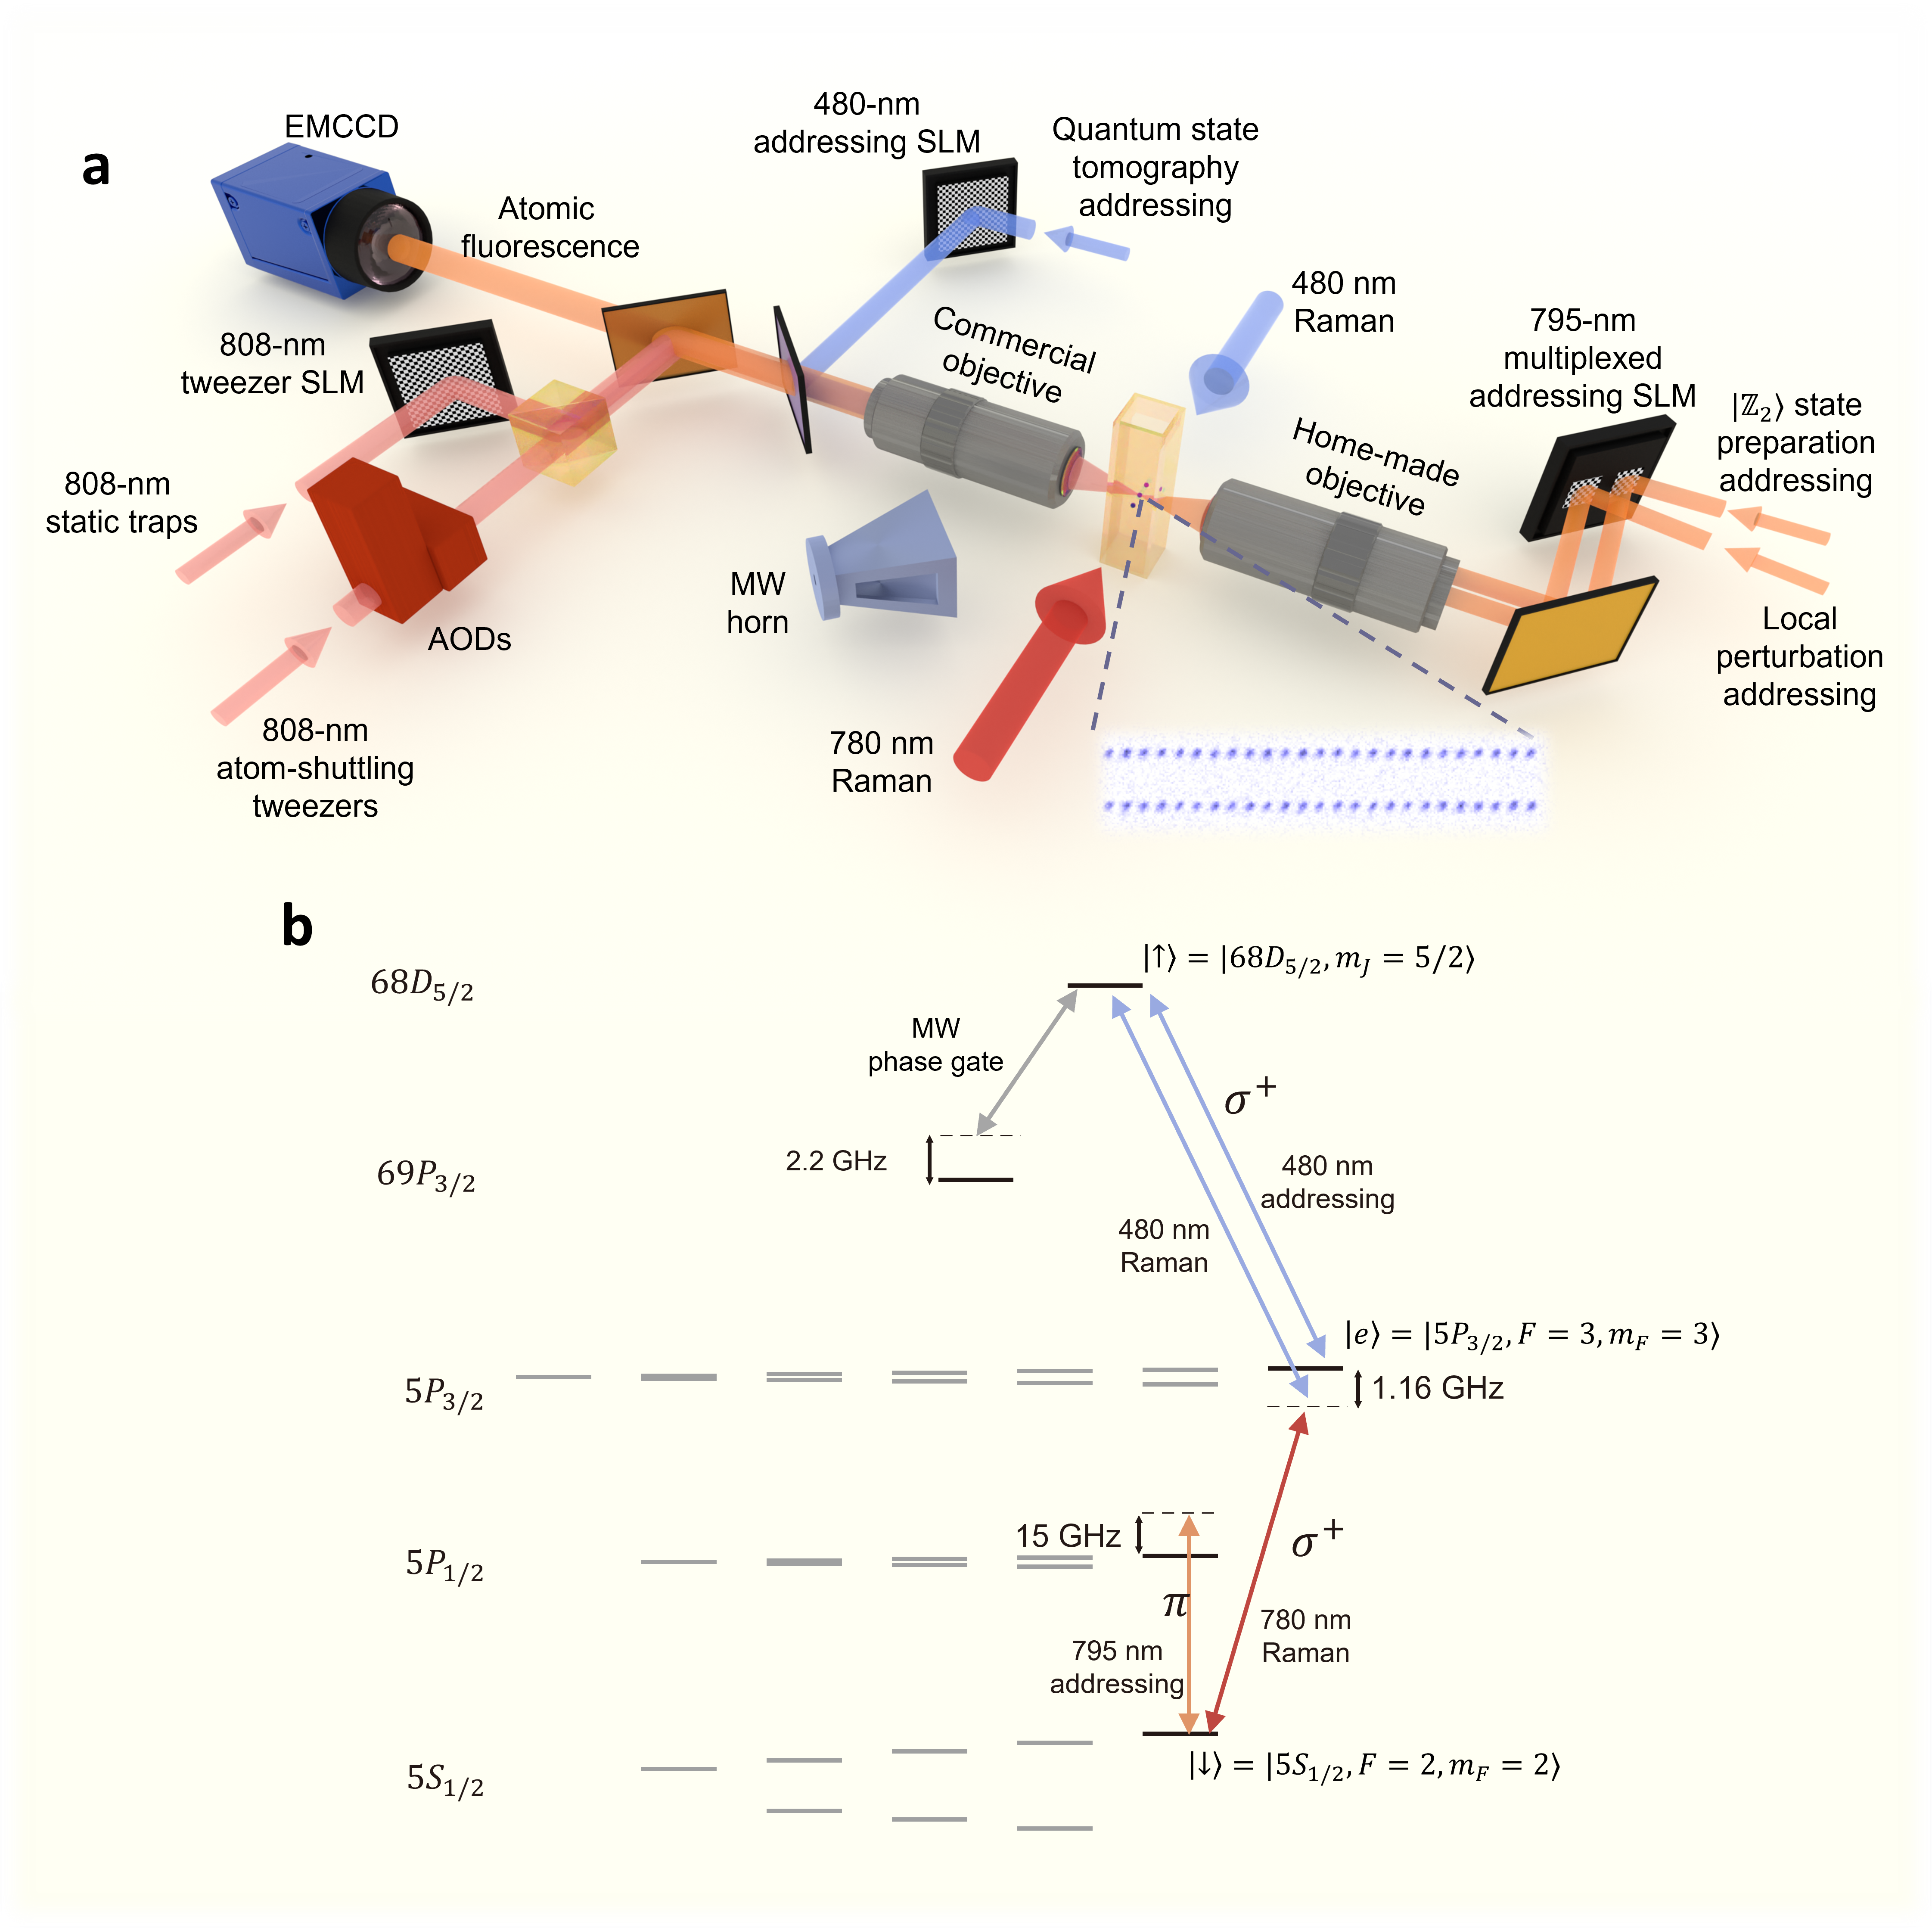
\includegraphics[width=0.7\textwidth]{figure_SI/Extended_Fig_1.png}  
  \caption{
    \textbf{实验装置和原子能级图。} 
    \textbf{a}, 实验装置中基本元件的示意图。808-nm 静态光镊由 SLM 产生,而原子运输光镊由两个声光偏转器 (AODs) 控制。480-\unit{\nano\meter} 寻址激光束由另一个 SLM 产生。商业物镜 (G Plan Apo 50$\times$, Mitutoyo, NA = 0.5) 聚焦 808-nm 光镊光束和 480-\unit{\nano\meter} 寻址光束,同时收集 795-\unit{\nano\meter} 原子荧光用于电子倍增 CCD (EMCCD) 相机上的成像。反向传播的 780-\unit{\nano\meter} 和 480-\unit{\nano\meter} 拉曼光束实现相干基态-里德堡操控。用于局域微扰 \(\hat\sigma_c^z\) 的 795-\unit{\nano\meter} 寻址激光和负责产生用于 $\ket{\mathbb{Z}_2}$ 态制备的交替光频移的激光阵列瞄准同一 SLM 的不同区域。这些不同区域显示不同的全息图,实现不同的寻址激光图案。这种空间复用技术允许在 \(\ket{\mathbb{Z}_2}\) 态制备和局域微扰激光配置之间进行亚微秒切换。795-\unit{\nano\meter} 寻址激光束通过自制物镜 (NA = 0.4) 聚焦到原子上。腔体附近的微波喇叭产生用于里德堡态操控(相位门)和探测的微波脉冲。插图显示了原子阵列。
    \textbf{b}, 显示实验中涉及的 $^{87}$Rb 原子能级的能级图。我们的里德堡激发方案采用从基态 \(\ket{\downarrow} = \ket{5S_{1/2}, F=2, m_F=2}\) 到里德堡态 \(\ket{\uparrow} = \ket{68D_{5/2}, m_J=5/2}\) 的双光子拉曼跃迁。该跃迁由 \(\hat\sigma^+\) 偏振的 780-\unit{\nano\meter} 激光(耦合基态到中间态 \(\ket{e}=\ket{5P_{3/2}, F=3, m_F=3}\))和 \(\hat\sigma^+\) 偏振的 480-\unit{\nano\meter} 激光(连接中间态到里德堡态)驱动。两束激光相对于中间态失谐 \(\Delta = 2\pi\times\SI{1.16}{\giga\hertz}\)。微波场相对于 \(\ket{\uparrow}\) 到 \(\ket{69P_{3/2}, m_J=3/2}\) 跃迁红失谐 $2\pi\times\SI{2.2}{\giga\hertz}$,在里德堡态上产生交流斯塔克频移,并提供用于反转 PXP 哈密顿量的相位门。对于局域单量子比特控制,采用相对于 \(\ket{\downarrow}\)-\(\ket{5P_{1/2}}\) 跃迁蓝失谐 $2\pi\times\SI{15}{\giga\hertz}$ 的 795-\unit{\nano\meter} 寻址光束,以及与 \(\ket{\uparrow}\)-\(\ket{e}\) 跃迁共振的 480-\unit{\nano\meter} 寻址光束。
    }
  \label{Fig:extended_1}
\end{figure*}

\begin{figure*}[!ht]
\centering
\includegraphics[width=0.8\textwidth]{figure_SI/Extended_Fig_Mitigated_exp_data.png}
\caption{\textbf{$\ket{\mathbb{Z}_2}$ 态的缓解 ZZ-OTOC 结果。} 
蓝点代表 $\ket{\mathbb{Z}_2}$ 态的缓解实验 ZZ-OTOC 数据,根据 IZ-OTOC 结果校正。
浅蓝曲线代表考虑了源于局域微扰 $\sigma^z_c$ 不完美的实验噪声的 PXP 哈密顿量 [式~(\ref{Eq:PXP})] 下的模拟 ZZ-OTOC 动力学。
深蓝曲线显示了里德堡哈密顿量 [式~(\ref{Rydberg Hamiltonian})] 下的模拟 ZZ-OTOC 动力学,也纳入了局域微扰 $\sigma^z_c$ 的不完美。
局域微扰中的不完美使得 OTOC 图案不太清晰,这无法使用 IZ-OTOC 缓解。
因此,这些不完美被纳入使用蒙特卡罗方法的数值模拟中(见补充材料第 4 节)。
}
\label{Mitigated_data}
\end{figure*}

\section{实验细节}
\label{section:experiment}
\LL{
可编程原子阵列已成为量子模拟和计算的新型平台,为探索量子多体现象提供了卓越的控制能力和可扩展性。
在过去十年中,该领域取得了显著进展,包括原子阵列的制备~\cite{piotrowicz2013two,endres2016atom,barredo2016atom,lee2017defect,barredo2018synthetic,kumar2018sorting,sheng2022defect,barnes2022assembly,okuno2022high,liu2023realization,pause2024supercharged},在量子计算~\cite{isenhower2010demonstration,jau2016entangling,sheng2018high,omran2019generation,guo2020balanced,bluvstein2022quantum,graham2022multi,fu2022high,schine2022long,singh2023mid,evered2023high,scholl2023erasure,ma2023high,zhao2023floquet,bluvstein2024logical,gregory2024second,shaw2024benchmarking}、量子优化~\cite{graham2022multi,ebadi2022quantum,kim2022rydberg,bluvstein2024logical}、量子模拟~\cite{bernien2017probing,keesling2019quantum,ebadi2021quantum,scholl2021quantum,semeghini2021probing,fang2024probing,DeLeseleuc2019,scholl2022microwave,chen2023continuous,kim2024realization}以及量子计量学~\cite{bornet2023scalable,eckner2023realizing}方面的努力。
本节介绍了我们实验的细节,包括实验装置、时序以及 $\ket{\mathbb{Z}_2}$ 态的制备和表征。
}



\subsection{实验装置}
\label{section:setup}

\LL{
本文的实验平台建立在双腔真空系统周围,由 2D 磁光阱 (MOT) 腔和科学腔组成。在 2D-MOT 腔中,$^{87}$Rb 原子源(安瓿)产生扩散的原子蒸气。这些原子被磁场和 780-\SI{}{\nano\meter} 激光冷却和束缚,激光相对于 $\ket{5S_{1/2}, F=2} \rightarrow \ket{5P_{3/2}, F=3}$ 循环跃迁红失谐 $2\pi\times \SI{30}{\MHz}$。预冷的原子系综随后通过差分泵浦孔径由 780-\SI{}{\nano\meter} 推送光束转移到科学腔中。
科学腔是一个定制设计的具有大光学通道的长方体玻璃腔 (Japan Cell)。腔内的超高真空条件由非蒸散型吸气剂泵 (NEXTorr D 200-5, SAES) 维持,实现了远低于 \(10^{-11}\) mbar 的压力。这种低背景压力最初允许单原子捕获寿命超过 10 分钟。然而,由于 2D-MOT 腔中离子泵 (SP-4, JJJvac) 的故障,寿命已降至约 \SI{90} 秒。原子在科学腔中被三维磁光阱 (3D-MOT) 捕获和冷却,使用三对反向传播的 780-\SI{}{\nano\meter} 激光束,磁场梯度为 \SI{15}{\gauss\per\cm}。每束光包含相对于 \(\ket{5S_{1/2}, F=2} \rightarrow \ket{5P_{3/2}, F=3}\) 循环跃迁红失谐 $2\pi\times \SI{24}{\MHz}$ 的冷却光,以及与 \(\ket{5S_{1/2}, F=1} \rightarrow \ket{5P_{3/2}, F=2}\) 跃迁共振的再泵浦光。
}

\LL{
单个原子被捕获在由 808-nm 激光器 (TA pro, Toptica) 在自由运行模式下产生的静态二维光镊阵列中。激光束照射加载了通过加权 Gerchberg-Saxton (WGS) 算法生成的相位全息图的相位控制空间光调制器 (SLM, HED 6010-NIR-080-C, Holoeye)。此外,一个原子运输光镊系统,利用与静态阵列相同的 808-nm 激光源但偏振正交,允许精确的原子重排。原子运输光镊由一对正交取向的声光偏转器 (AODs, DTSX-400-800.850, AA Opto-Electronic) 控制,由双通道任意波形发生器 (AWG, M4i.6631-x8, Spectrum) 生成的具有独立任意波形的射频驱动。
}

\LL{高数值孔径物镜 (G Plan Apo 50$\times$, Mitutoyo, NA = 0.5) 聚焦静态和可移动光镊,同时收集原子荧光,荧光被引导到电子倍增 CCD (EMCCD, iXon Ultra 888, Andor) 相机进行探测。此外,用于局域里德堡控制的 480-\SI{}{\nano\meter} 光束,利用类似的基于 SLM 的方法,通过同一物镜聚焦(见图~5a)。这种用于捕获、寻址和荧光探测的共享配置增强了系统的稳定性。}
\LL{
与 Mitutoyo 物镜相对的是一个数值孔径为 0.4 的自制物镜。CCD 相机对静态光镊阵列成像,该阵列由 36 \(\times\) 2 个光镊组成,间距为 \SI{7}{\um},束腰约为 \SI{0.9}{\um}。通过迭代反馈和调整,整个阵列的强度变化保持在 1\% 以下。对于 \(\ket{\mathbb{Z}_2}\) 态制备和局域微扰至关重要的 795-\SI{}{\nano\meter} 寻址激光束通过自制物镜聚焦。两束反向传播的激光束——一束在 \SI{780}{\nm},另一束在 \SI{480}{\nm}——实现全局基态-里德堡相干操控。位于科学腔附近的微波天线产生用于里德堡态操控和探测的微波脉冲。
}

\LL{
实验装置集成了用于态制备、量子比特控制和探测的多个激光系统。780-\SI{}{\nano\meter} 激光系统,一个锥形放大器激光器 (TA Pro, Toptica),用于 MOT 冷却光束和里德堡激发方案中的拉曼光。其频率被稳定到精细度为 26,000 的超低膨胀参考腔 (SLS)。AWG 驱动针对调制带宽进行了优化的单次通过声光调制器 (AOM, SGT200-780-0.5TA-B),以动态调整脉冲频率和强度。
为了耦合 \(\ket{e} \rightarrow \ket{r}\) 跃迁,采用了 480-\SI{}{\nano\meter} 激光系统(倍频 TA-SHG Pro, Toptica),960-nm 种子激光器锁定到与 780-\SI{}{\nano\meter} 激光器相同的参考腔。由直接数字合成 (DDS, AD9910) 驱动的 AOM 控制 480-\SI{}{\nano\meter} 激光束,该光束经过强度稳定并在整个里德堡操作序列中保持开启。里德堡激发激光的快速上升和下降沿是使用电光调制器 (EOMs) 实现的,以进行精确的开关切换。
}

\begin{figure}
  \centering
  \includegraphics[width=\textwidth]{figure_SI/compressed/SI_Timing_sequence.png}  
  \caption{
    \textbf{实验时序。} 
    如第~\hyperref[section:timing sequence]{1.2} 节所述的典型实验序列总结。用于 OTOC 和 Holevo 信息测量的详细里德堡实验序列在图~\ref{SI_OTOC_sequence},\ref{SI_HI_sequence} 中提供。
    }
  \label{Fig:S1}
\end{figure}




\subsection{实验时序} 
\label{section:timing sequence}



\LL{
实验序列开始于在科学腔中制备冷原子系综。3D MOT 加载 \SI{200}{\ms},产生直径为 \SI{500}{\um}、温度为 \SI{150}{\micro\kelvin} 的原子云,通过飞行时间 (TOF) 膨胀测量。为了进一步降低温度,应用了偏振梯度冷却 (PGC)。该过程涉及快速关闭磁场梯度(在 \SI{500}{\us} 内),同时将冷却光失谐增加到约 $2\pi\times\SI{90}{\MHz}$ 并降低冷却和再泵浦激光的强度。结果,原子被进一步冷却至约 \SI{40}{\micro\kelvin}。
}
\LL{
激光冷却的原子系综作为随机加载可编程原子阵列的库。对于随机加载,使用两束反向传播的 795-\SI{}{\nano\meter} 激光束实施 \(\Lambda\) 增强灰光学粘团 (\(\Lambda\)GM)。
随后应用针对阱内冷却优化的额外偏振梯度冷却 (PGC) 阶段。这种组合冷却方法导致单原子加载效率约为 80\%,在深度为 \SI{1}{\milli\kelvin} 的阱中平均原子温度为 \SI{15}{\micro\kelvin},这是使用释放-再捕获 (R\&R) 方法测量的。原子荧光探测利用用于 \(\Lambda\)GM 的相同 795-\SI{}{\nano\meter} 光束,在将光阱深度增加到 \SI{1.3}{\milli\kelvin} 后进行复用。通过仔细平衡加热和冷却速率,在 \SI{30}{\ms} 曝光时间内实现了超过 99.9\% 的探测保真度,同时保持每次探测的平均原子损失低于 1\%。使用 795-\SI{}{\nano\meter} 荧光成像最小化了来自强 780-\SI{}{\nano\meter} 光束的串扰,确保了准确的原子探测。
}

\LL{
原子重排过程产生无缺陷的一维原子链。该过程开始于将可移动光镊的强度从零线性增加到静态阱深度的三倍,将原子从静态 SLM 生成的阱转移到可移动光镊。然后用含时波形驱动 AODs 以平均速度 \SI{100}{\um\per\ms} 运输原子,遵循正弦速度分布以确保平滑的加速和减速。重排序列是使用改进的匈牙利算法 \cite{lee2017defect} 确定的,逐列优化原子移动。为了最小化移动光镊扫过静态阱时不必要的原子损失和加热,光镊路径包括额外的段以绕过中间的阱。重排过程的所有 AOD 波形都是预先计算的,允许快速执行序列。重排后测量表明,在 \SI{1}{\milli\kelvin} 深的阱中,原子温度增加到约 \SI{50}{\micro\kelvin}。
}

\LL{
对于相干里德堡激发,采用双光子拉曼方案。具有 \(\sigma^+\) 偏振的红失谐 780-\SI{}{\nano\meter} 激光将基态耦合到中间态 \(\ket{5P_{3/2}, F=3, m_F=3}\)(见图~5b)。准直的 780-\SI{}{\nano\meter} 激光被引导到原子上,束腰约为 \SI{300}{\um},最大拉比频率为 \(\sim 2\pi\times\SI{100}{\MHz}\)。同时,同样具有 \(\sigma^+\) 偏振的蓝失谐 480-\SI{}{\nano\meter} 激光将中间态连接到里德堡态 \(\ket{\uparrow} = \ket{68D_{5/2}, m_J=5/2}\)。480-\SI{}{\nano\meter} 激光聚焦到原子上,束腰为 \SI{13}{\um},最大拉比频率为 \(\sim 2\pi\times\SI{70}{\MHz}\)。两束激光相对于中间态失谐 \(\Delta = 2\pi\times\SI{1.16}{\GHz}\)。
整个实验过程中施加 \SI{30}{\gauss} 的偏置磁场。
图~\ref{SI_Block_Rabi}a(蓝色圆圈)展示了由 780-\SI{}{\nano\meter} 和 480-\SI{}{\nano\meter} 激光驱动的单个原子的高对比度基态-里德堡态拉比振荡。当两个原子位于里德堡阻塞区域内时,$\Omega \ll V$,双里德堡激发受到强烈抑制,如图~\ref{SI_Block_Rabi}a 中的黄色方块所示。图~\ref{SI_Block_Rabi}a 中的红色菱形显示,贝尔态 $\frac{1}{\sqrt{2}}(\ket{\downarrow}\ket{\uparrow}+\ket{\uparrow}\ket{\downarrow})$ 和基态 $\ket{\downarrow}\ket{\downarrow}$ 之间的拉比振荡增强了 \(\sqrt{2}\) 倍。图~\ref{SI_Block_Rabi}b 展示了单个原子的基态-里德堡相干性,其中我们执行两个由可变间隙隔开的 \(\pi/2\) 基态-里德堡旋转,以实施 Ramsey 序列。Ramsey 振荡条纹的衰减揭示了 $T^*_2=\SI{11(1)}{\us}$ 的基态-里德堡相干时间。在我们的系统中实现的高对比度拉比振荡和长相干时间为后续实验中的高保真度操作奠定了坚实的基础。
}


\begin{figure}[t]
  \centering
  \includegraphics[width=0.9\textwidth]{figure_SI/compressed/SI_Block_Rabi.png}  
  \caption{
\textbf{基态-里德堡态拉比振荡、里德堡阻塞和 Ramsey 相干性。} 
\LL{
\textbf{a}, 当单个原子由 480-\SI{}{\nano\meter} 和 780-\SI{}{\nano\meter} 拉曼激光驱动时,观察到高对比度基态-里德堡态拉比振荡(蓝色圆圈)。对于阻塞半径内的一对原子,双里德堡激发(黄色方块)受到强烈抑制,并且由于里德堡阻塞效应,单激发的拉比频率(红色菱形)增强了 \(\sqrt{2}\) 倍。曲线是阻尼正弦拟合。
\textbf{b}, Ramsey 振荡显示高斯型非均匀退相,相干时间为 \(T^*_2 = \SI{11(1)}{\micro\second}\)。测量的概率代表间隙时间后的 \(\frac{1}{2}(\langle \sigma^y \rangle + 1)\)。
}
}
  \label{SI_Block_Rabi}
\end{figure}

\LL{
为了在基态和里德堡态上执行局域操作,我们采用由 SLM 生成的 795-\SI{}{\nano\meter} 和 480-\SI{}{\nano\meter} 寻址激光束。795-\SI{}{\nano\meter} 激光束相对于 \(\ket{5S_{1/2}, F=2} \rightarrow \ket{5P_{1/2}}\) 跃迁蓝失谐 \(2\pi \times \SI{15}{\GHz}\),提供 \(2\pi \times \SI{12.2(3)}{\MHz}\) 的光频移。这使得能够创建可激发和不可激发原子的交替图案,允许系统被制备在 $\mathbb{Z}_2$ 有序配置中。
在 EMCCD 上同时对 795-\SI{}{\nano\meter} 原子荧光和 795-\SI{}{\nano\meter} 寻址激光束成像,确保了激光和原子之间的精确空间重叠。测量表明,对链中相邻原子的串扰被抑制到低于 \(2\pi \times \SI{1}{\kHz}\)。
与 $\ket{r}-\ket{e}$ 跃迁共振的 480-\SI{}{\nano\meter} 激光束用于实现选择性里德堡-基态转移,并在最近邻 (NN) 和次近邻 (NNN) 格点中创建 EIT 条件。480-\SI{}{\nano\meter} 激光束对准通过最大化目标格点上的里德堡-基态转移效率同时最小化相邻格点上的串扰来优化。优化后,目标格点中超过 96\% 的里德堡态布居被快速转移到基态,而相邻格点中的里德堡态布居减少不到 1\%。
}

\LL{
最后,实施态探测方案以区分基态和里德堡态。在里德堡操作后 \SI{1}{\us} 内,阱深度迅速增加到 \SI{1.3}{\milli\kelvin} 以将里德堡原子从捕获区域排出,同时重新捕获基态原子。随后,使用射频功率放大器 (HXPA7081G, HXINWB) 施加扫描强 \SI{2.4}{\GHz} 微波脉冲以耗尽剩余的里德堡布居。这种综合探测方案确保了将里德堡原子误识别为基态的概率小于 1\%。
}


\subsection{$\ket{\mathbb{Z}_2}$ 态制备和表征}
\label{section:Z2}

\begin{figure}
  \centering
  \includegraphics[width=\textwidth]{figure_SI/compressed/SI_Z2.png}  
  \caption{
    \textbf{$\ket{\mathbb{Z}_2}$ 态制备细节。} 
    \textbf{a}, \LL{被寻址(红色)和未被寻址(蓝色)原子的里德堡激发光谱。里德堡布居显示为拉曼激发激光失谐的函数。}
    \textbf{b}, \LL{反阻塞效应和寻址激光诱导的光频移对态制备保真度的影响。模拟的 $\ket{\mathbb{Z}_2}$ 态制备保真度作为 795-\SI{}{\nano\meter} 寻址激光光频移(以里德堡拉曼激发拉比频率 $\Omega$ 为单位)的函数,针对各种系统尺寸,最近邻里德堡相互作用强度 $V_{i,i+1}=3\Omega$。红星标记了我们的实验条件。}
    \textbf{c}, \LL{$\ket{\mathbb{Z}_2}$ 态制备保真度作为系统尺寸的函数。红线和蓝线:校正和未校正 $\ket{\mathbb{Z}_2}$ 态保真度的指数拟合。黄线:当前实验寻址方法的理论上限。}
    \textbf{d}, \LL{13 量子比特微观态数量作为来自 1,774 次实验的出现次数的函数。成功制备的 $\ket{\mathbb{Z}_2}$ 态:1,246 次计数(70\% 的事件)。}
    \textbf{e}, \LL{测量的 13 量子比特微观态分布。插图:主要错误态。}
  }
  \label{Fig:S2}
\end{figure}


\LL{
快速热化在遍历量子多体系统中普遍存在,导致旨在发现具有根本不同动力学的系统的大量研究~\cite{deutsch1991quantum,srednicki1994chaos,rigol2008thermalization,deutsch2018eigenstate,lewis2019dynamics}。
% swingle2018unscrambling, abanin2019colloquium
最近,涉及里德堡原子阵列的研究已经确定了多体疤痕态~\cite{bernien2017probing,turner2018weak,choi2019emergent,ho2019periodic,bluvstein2021controlling,turner2021correspondence,serbyn2021quantum},这些态表现出遍历性的弱破坏,并在延长的时标上保持一定程度的相干性。\ZYW{类似的现象已在其他系统中观察到,例如超导处理器~\cite{zhang2023many}和玻色-哈伯德量子模拟器~\cite{su2023observation},并引发了进一步的理论研究~\cite{maskara2021discrete,dong2023disorder,liu2024novel, desaules2024ergodicity, aron2024quantum}。}
先前的理论工作~\cite{yuan2022quantum}预测,当使用 $\mathbb{Z}_2$ 有序奈尔态作为研究反时序关联函数和 Holevo 信息时空演化的初态时,可能会观察到持续的信息回流和量子混沌的不寻常破坏。这些结果表明了研究动力学受限多体系统中量子信息加扰独特动力学的新途径。
在此,本文使用两种初态研究量子信息加扰:(1) $\mathbb{Z}_2$ 有序态 \(\ket{\mathbb{Z}_2} = \ket{\uparrow \downarrow \uparrow \downarrow \uparrow...}\) 和 (2) 平凡直积态 \(\ket{\mathbf{0}} = \ket{\downarrow \downarrow \downarrow \downarrow \downarrow...}\)。虽然 \(\ket{\mathbf{0}}\) 可以很容易地使用光泵浦制备,但在大规模系统中实现 \(\ket{\mathbb{Z}_2}\) 态的高保真度制备仍然具有挑战性。
先前的研究已经通过绝热态转移技术在一维和二维原子阵列中成功制备了 \(\ket{\mathbb{Z}_2}\) 态~\cite{bernien2017probing,omran2019generation,bluvstein2021controlling},其中设计哈密顿量的基态从 \(\ket{\mathbf{0}}\) 绝热变换为 \(\ket{\mathbb{Z}_2}\)。然而,随着系统尺寸的增加,希尔伯特空间的指数增长导致能隙减小,这导致态制备保真度的迅速下降。
}

\LL{
本文的实验采用了一种可扩展的态制备方法,结合了全局里德堡激发和格点选择性激光寻址。SLM 用于在原子阵列上产生定制的光频移图案,选择性地使某些格点从基态-里德堡跃迁失谐(图~\ref{Fig:S2}a),从而创建可激发和不可激发原子的交替排列。
795-\SI{}{\nano\meter} 寻址光束,相对于 D1 线共振失谐 $2\pi \times \SI{15}{\GHz}$,在基态上诱导 $2\pi \times \SI{12.2(3)}{MHz}$ 的能量移动。由 795-\SI{}{\nano\meter} 寻址光束引起的散射率约为 $2\pi \times \SI{5}{kHz}$,明显低于拉曼激光束引起的散射率。数值模拟(图~\ref{Fig:S2}b)表明,为了最大化 \(\ket{\mathbb{Z}_2}\) 态的保真度,光频移的符号必须与里德堡相互作用的符号相反,以避免反阻塞效应。在我们的实验条件下,数值模拟产生的制备非保真度约为每个量子比特 0.012。
}

\LL{
我们的方法在系统尺寸扩大时仍然非常有效(图~\ref{Fig:S2}c)。制备非保真度主要归因于不相关的单量子比特翻转误差:来自里德堡激发低效率的每个量子比特 0.8\%,由于有限能量移动的每个量子比特 1.2\%,以及来自态探测误差的 1\% ($\ket{\downarrow}\rightarrow\ket{\uparrow}$) 和 0.5\% ($\ket{\uparrow}\rightarrow\ket{\downarrow}$)。
%of many-body scar state preparation 
这种分解为单量子比特态制备的方式
增强了我们方法相对于绝热转移协议的可扩展性。
在多达 25 个原子的阵列中,我们实现了目标 $\ket{\mathbb{Z}_2}$ 态,测量保真度为 49(3)\%,在考虑探测误差后校正为 60(3)\%。在 $2^{25}$ 维的希尔伯特空间中的这种高保真度制备强调了我们协议的鲁棒性和可扩展性。
}

\LL{
实验制备的 $\ket{\mathbb{Z}_2}$ 态的微观态分布分析揭示了非泊松误差发生(图~\ref{Fig:S2}d)。
图~\ref{Fig:S2}e 显示了测量的微观态分布,突显了主要误差是从 $\ket{\uparrow}$ 到 $\ket{\downarrow}$ 的单量子比特翻转,进一步证实了我们的方法采用单量子比特操作来制备多体态。这种可预测的误差分布有助于在 $\ket{\mathbb{Z}_2}$ 态中量子信息加扰的实验测量数据中进行误差缓解,如第~\ref{section:error} 节所讨论的。
}

\LL{接下来,研究了 $\ket{\mathbb{Z}_2}$ 态的演化和寿命。$\ket{\mathbb{Z}_2}$ 态的动力学是在使用 PXP 哈密顿量 \(H = \sum_i P_i \sigma^x_{i+1} P_{i+2}\)~\cite{lesanovsky2012interacting,turner2018weak,cheng2024emergent} 的正向-反向演化(\(e^{-iHt}\) 后跟 \(e^{iHt}\))和仅正向演化(\(e^{-iHt}\))(图~\ref{Fig:S3})下测量的。为了表征演化,测量了里德堡态布居 \(P(\uparrow)\)(图~\ref{Fig:S3}a,b)和平均畴壁密度(图~\ref{Fig:S3}c,d)。
图~\ref{Fig:S3}a,c 中数据的指数拟合显示了 $\ket{\mathbb{Z}_2}$ 态在正向-反向演化下的衰减率,布居的 $1/e$ 寿命约为 \SI{1.6(1)}{\micro\second},平均畴壁密度为 \SI{1.0(3)}{\micro\second}。这种衰减限制了正文图 3f 中呈现的原始 ZZ-OTOC 数据的对比度。平均畴壁密度的仅正向演化(图~\ref{Fig:S3}d)拟合为阻尼正弦函数,产生约 \SI{1.5(1)}{\micro\second} 的 $\ket{\mathbb{Z}_2}$ 态寿命。
\LL{
里德堡布居动力学(图~\ref{Fig:S3}b)使用阻尼傅里叶级数拟合,产生约 \SI{2.8(2)}{\us} 的 $1/e$ 衰减时间。
}
此外,在第~\ref{section:error} 节中,来自图~\ref{Fig:S3}b 的数据被拟合到误差模型以表征驱动场中的噪声。$\ket{\mathbb{Z}_2}$ 态的有限寿命导致传输过程中的整体损失,反映在正文图 4b 中测量的 Holevo 信息的全局衰减中。
无缺陷 $\mathbb{Z}_2$ 有序系统分解为子系统,由畴壁密度的衰减(图~\ref{Fig:S3}c)和振荡对比度的降低(图~\ref{Fig:S3}d)表明,这模糊了动力学并阻碍了量子信息传播。
虽然态制备误差可以很容易地校正,但演化过程中误差的缓解要复杂得多。上述对制备的 $\ket{\mathbb{Z}_2}$ 态的详细表征,特别是驱动演化期间的衰减率,提供了对潜在噪声源的见解(关于噪声模型的细节见第~\ref{section:error} 节),并为随后的误差缓解策略提供信息。}



\LL{
总之,演示了一种在大型原子阵列中制备 $\ket{\mathbb{Z}_2}$ 态的可扩展方法。通过结合全局里德堡激发和格点选择性寻址,在多达 25 个量子比特的系统中实现了高保真度态制备。态演化的详细表征提供了对量子疤痕动力学和系统噪声源的宝贵理解。这些发现为进一步探索疤痕系统中的量子信息加扰奠定了基础。
}


\begin{figure}
  \centering  \includegraphics[width=0.75\textwidth]{figure_SI/compressed/SI_lifetime.png}  
  \caption{
\textbf{PXP 哈密顿量演化下的 $\ket{\mathbb{Z}_2}$ 态动力学。} 
\LL{
\textbf{a} 和 \textbf{b}, 初始化量子比特在 \textbf{a}, 正向-反向演化 \((e^{-iHt}\) 后跟 \(e^{iHt})\) 和 \textbf{b}, 仅正向 \((e^{-iHt})\) 演化期间的 \(\ket{\uparrow}\)(蓝色)和 \(\ket{\downarrow}\)(红色)布居。 \textbf{a} 中的曲线代表指数拟合,
%with a shared offset and decay rate \ZYW{yielding a 1/e lifetime of \SI{1.57(6)}{\micro\second}
而 \textbf{b} 用高达 5 阶的阻尼傅里叶级数拟合。
%The damping rate for each order is set to the same, which yields a 1/e lifetime of \SI{2.8(2)}{\micro\second}.} 
\textbf{c} 和 \textbf{d}, 中心 13 个量子比特在 \textbf{c}, 正向-反向演化和 \textbf{d}, 仅正向演化期间的平均畴壁密度 (DWD)。\textbf{c} 中的蓝色曲线是指数拟合,
%with a 1/e lifetime of \SI{1.61(11)}{\micro\second}, 
而 \textbf{d} 拟合为阻尼正弦函数。
%yielding a lifetime of \SI{1.47(8)}{\micro\second}.
}
}
  \label{Fig:S3}
\end{figure}

\section{理论建模与数值模拟}

\subsection{有效哈密顿量和数值模拟方法}


\LL{我们的实验装置由一个被光镊捕获的 25 个单个原子的线性阵列组成。系统动力学由微观哈密顿量支配:
\begin{equation}
H = \sum_i \left[\frac{\Omega}{2} \sigma^x_i - \Delta n_i \right] + \sum_{i<j} V_{ij} n_i n_j,
\label{eq:rydberg_hamiltonian}
\end{equation}
其中 $\Omega$ 是拉比频率,$\Delta$ 是失谐,$n_j = (1 + \sigma^z_j)/2$ 是格点 $j$ 上向 $\ket{\uparrow}$ 的投影算符,指示原子是否处于里德堡态。相互作用项 $V_{ij} = C_6/R^6_{ij}$ 代表位于格点 $i$ 和 $j$ 处于 $\ket{\uparrow}$ 态的原子之间的范德瓦尔斯相互作用,其中 $C_6$ 是范德瓦尔斯系数,$R_{ij}$ 是原子间的距离。}

\LL{在强最近邻相互作用区域($\Omega \ll V_{i,i+1}$),忽略长程相互作用($V_{i,j>i+1}$),并设定失谐 $\Delta = 0$,哈密顿量通过施里弗-沃尔夫变换简化为有效 PXP 哈密顿量:
\begin{equation}
H_\text{PXP} = \sum_i P_i \sigma^x_{i+1} P_{i+2},
\label{eq:pxp_hamiltonian}
\end{equation}
其中 $P_i = (1 - \sigma^z_i)/2$ 是格点 $i$ 上向 $\ket{\downarrow}$ 态的投影算符,$\sigma^{x,y,z}_i$ 是第 $i$ 个量子比特的泡利矩阵。
局域三体项 $P_i \sigma^x_{i+1} P_{i+2}$ 施加动力学约束,允许里德堡原子态仅在两个相邻原子都处于自旋向下 $\ket{\downarrow}$ 态时才翻转。这个约束有效地从计算基中排除了配置 $\ket{\cdots \uparrow_i\uparrow_{i+1}\cdots}$,因为相邻里德堡激发被阻塞效应禁止。
由没有相邻激发态的配置张成的低能子空间可以由投影算符描述:
\begin{equation}
\mathcal{P} = \prod_j \left( 1 - n_j n_{j+1}\right).
\label{eq:projector}
\end{equation}
这个受限子空间形成了维度降低的有效希尔伯特空间,支配着系统的受限动力学。值得注意的是,这个有效希尔伯特空间的维度按照斐波那契数列增长,缩放为 $\phi^N$,其中 $\phi = (1+\sqrt{5})/2$ 是黄金分割比,$N$ 是系统尺寸。
这种维度降低反映了由于动力学约束而排除某些配置。}

\LL{PXP 模型表现出三种显著的对称性:
(1) 离散空间反演对称性 $\mathcal{I}$,映射 $j \rightarrow N-j+1$。
(2) 平移对称性,适用于周期性边界条件。
(3) 粒子-空穴对称性,由 $\mathcal{C} = \prod_j \sigma_j^z$ 表示,导致 $\mathcal{C} H_\text{PXP}\mathcal{C} = -H_\text{PXP}$。
粒子-空穴对称性在我们实验中反转哈密顿量演化 $\text{exp}(-iH t)$ 中起着至关重要的作用。然而,这种对称性仅存在于 PXP 哈密顿量 $H_\text{PXP}$ 中,而不存在于支配实验的完整里德堡哈密顿量 $H$ 中,这导致了时间反演的不完美。}

\LL{当初始化在 $\ket{\mathbb{Z}_2}$ 态时,里德堡原子系统表现出具有缓慢衰减的波函数振荡。这种衰减部分归因于实验演化过程中的态丢失和退相干,但也源于多体疤痕的不完美以及与基础 PXP 模型中热态的小重叠。
为了更好地理解内在动力学对观察到的衰减的贡献,我们对复苏行为进行了数值模拟,将尺寸 $N=25$ 的系统初始化在 $\ket{\mathbb{Z}_2}$ 态。结果如图~\ref{Fig:SI_toy}c 所示,提供了证据表明观察到的衰减的很大一部分可以归因于 PXP 模型的内在特征。}

\begin{figure}[t]
\centering
\includegraphics[width=0.7\textwidth]{figure_SI/compressed/SI_experimental_parameters.png}
\caption{\textbf{优化实验参数以紧密近似理想 PXP 哈密顿量动力学。} 
\LL{具有周期性边界条件的 10 量子比特链中中心量子比特的 OTOC 和时间反演保真度的数值模拟。\textbf{a}, 模拟的不同最近邻 (NN) 里德堡相互作用 $V_{i,i+1}$ 下的 OTOC 动力学,与理想 PXP 模型进行比较。相互作用强度从 $2\Omega$ 变化到 $10\Omega$,步长为 $2\Omega$。最佳选择 $V_{i,i+1} = 6\Omega$ 最匹配理想情况。
\textbf{b}, 时间反演保真度作为拉比频率 $\Omega$ 的函数,其中 $V_{i,i+1}$ 固定为 $6\Omega$。显示了 $\Omega t = 1.0\pi$(蓝色符号)、$\Omega t = 1.5\pi$(黄色符号)和 $\Omega t = 2.0\pi$(红色符号)的不同时间演化。随着 $\Omega$ 增加,保真度降低。
\textbf{c}, 不同失谐值 $\Delta$ 下的 OTOC 动力学,范围从 $\Delta = 0$ 到 $3V_{i,i+2}$,其中 $V_{i,i+2}$ 是次近邻 (NNN) 相互作用。黑色曲线代表理想 PXP 模型。最佳失谐 $\Delta = 2V_{i,i+2}$ 最匹配理想动力学。
\textbf{d}, 使用优化实验参数(紫色曲线)和理想 PXP 模型(黑色曲线)的 OTOC 动力学比较,显示出紧密一致。优化参数有效地再现了 OTOC 中观察到的关键振荡。}

} 
\label{FIG:experimental parameters}
\end{figure}


\LL{对于所有数值模拟,我们采用里德堡哈密顿量 (\ref{eq:rydberg_hamiltonian}) 来紧密近似实验物理条件。对于长度 $\leq$ 13 的原子链,我们利用精确对角化来高效计算完整的时间演化。然而,对于超过 13 个原子的链,由于指数增加的内存需求和计算时间,以及可用计算资源的限制,精确对角化在计算上变得不可行。因此,我们在这些情况下实施矩阵乘积算符 (MPO) 方法来加速我们的数值计算。这种方法允许我们将模拟扩展到更长的原子链,同时利用 TeNPy 保持计算可行性和数值精度~\cite{Johannes2018Efficient}。除非另有说明,所有模拟采用与实验设置相同的参数(详见第 \ref{section:experiment} 节)。为了考虑实验不确定性,我们实施蒙特卡罗方法:考虑拉比频率和失谐的波动、激光噪声、原子位置的不确定性以及其他相关实验参数,所有变量均从其各自的概率分布中随机采样。通常,我们执行 200 次运行并平均结果。这种综合方法提供了在现实实验条件下系统行为的稳健表示。}

\subsection{最佳量子动力学的参数调节}

\label{section:experimental parameter}

\LL{有效 PXP 哈密顿量的近似依赖于两个关键假设:
(1) 忽略长程相互作用 $V_{i,j>i+1}$。
(2) 确保最近邻相互作用主导拉比频率($V_{i,i+1} \gg \Omega$)。}

\LL{然而,实际上,次近邻相互作用 $V_{i,i+2}$ 不能被忽略。为了紧密近似 PXP 模型,系统必须在 $V_{i,i+2} \ll \Omega \ll V_{i,i+1}$ 的区域运行。这是一个挑战,因为在我们具有等间距原子的一维几何结构中,比率 $V_{i,i+1}/V_{i,i+2}$ 固定在约 64。例如,设置 $V_{i,i+1} \sim 16\Omega$ 以满足第二个假设会导致 $\Omega \sim 4V_{i,i+2}$,使得难以完全抑制 $V_{i,i+2}$ 的影响。这在两个关键假设之间产生了权衡。}

\LL{为了找到 $V_{i,i+1}/\Omega$ 的最佳比率,我们对不同参数下的 ZZ-OTOC 进行了数值模拟。我们确定了最小化\R{\sout{塌缩与复苏}振荡对比度}衰减的最佳比率,如图~\ref{FIG:experimental parameters}a 所示。基于这些结果,我们将 $V_{i,i+1}/\Omega$ 的实验比率设置为 6,这与理论中间值 $\Omega=\sqrt{V_{i,i+1} V_{i,i+2}}$ 不同。}

\LL{拉比频率的选择涉及平衡两个相互竞争的因素:(1) 时间反演保真度:我们的模拟(图~\ref{FIG:experimental parameters}b)表明,当 $V_{i,i+1}/\Omega$ 固定为 6 且正向和反向演化之间的间隔固定为 \SI{200}{\nano\second} 时,增加拉比频率会降低时间反演保真度。(2) 单原子相干性:较高的拉比频率提高了主要受激光相位噪声限制的单原子相干性。}

\LL{在仔细权衡这些因素后,我们选择了 $\Omega = 2\pi \times \SI{1.21(1)}{MHz}$ 的拉比频率。该值在保持足够的时间反演保真度和确保满足我们实验需求的足够单原子相干性之间取得了平衡。}

\LL{除了优化 $V_{i,i+1}$ 和 $\Omega$ 外,我们还引入了一个小的失谐 $\Delta$ 来抵消残留的次近邻相互作用 $V_{i,i+2}$。我们的模拟表明,设置 $\Delta = 2V_{i,i+2}$ 最能捕捉 OTOC \R{\sout{塌缩与复苏现象} 动力学}(图~\ref{FIG:experimental parameters}c)。
}


\LL{
在我们的 OTOC 测量中,在正向和反向演化之间插入了一个间隙,用于实施局域和全局单量子比特 $\sigma^z$ 操作。
为了将间隙时间最小化到 $\sim$ \SI{200}{ns},我们并行执行局域微扰和全局 $\sigma^z$ 旋转,利用它们的对易性质。我们数值研究了这个有限间隙对实验中观察到的\R{\sout{信息塌缩与复苏行为} OTOC 动力学}的影响,如图~\ref{FIG:experimental parameters}d 所示。我们的分析表明,实验中使用的 \SI{200}{ns} 单量子比特操作时间不会显著影响\R{\sout{塌缩与复苏现象} 振荡行为的观测}。
}

\LL{
这些参数优化使我们能够在实验装置中紧密近似 PXP 模型(图~\ref{FIG:experimental parameters}d),尽管我们的系统存在固有约束。
这些结果突显了精确参数调节对于准确实现目标哈密顿量和最大化里德堡原子系统中量子多体疤痕演化保真度的重要性。优化后的参数促进了动力学约束下相干自旋旋转动力学的实验实现,紧密近似 PXP 模型的理想行为。}



\subsection{边界和有限尺寸效应}
\label{section:boundary}

\LL{在有限尺寸量子比特链中,边界量子比特的存在打破了 PXP 哈密顿量对于某些初态如 $\ket{\mathbb{Z}_2} = \ket{...\uparrow \downarrow\uparrow\downarrow\uparrow...}$ 和 $\ket{\mathbf{0}} = \ket{...\downarrow \downarrow\downarrow\downarrow\downarrow...}$ 的平移对称性。这种对称性破缺导致边缘和体量子比特之间的相互作用强度不同(图~\ref{Fig:Boundary and finite-size effect}a),引入显著的边界效应。此外,有限的粒子数导致体原子在不同系统尺寸下的动力学演化存在差异,引入有限尺寸效应。对于包含长程相互作用的里德堡哈密顿量,由于边缘与体相比残留相互作用的差异,这些边界效应进一步放大。}

\LL{为了定量分析边界效应,我们数值模拟了 13 量子比特链中中心和边缘量子比特的演化动力学,从理想里德堡哈密顿量下的 $\ket{\mathbb{Z}_2}$ 态开始。如图~\ref{Fig:Boundary and finite-size effect}b,c 所示,边界效应导致边缘量子比特表现出加速的周期性振荡。这种加速源于对边缘量子比特的约束减少,导致更强的有效驱动强度。}

\LL{此外,数值模拟和实验结果都表明,边界效应逐渐从外边缘向内改变自旋旋转,导致最初均匀传播的波前在 $\ket{\mathbb{Z}_2}$ 初态的演化过程中发生弯曲,强调了边界效应在塑造系统动力学中的关键作用。}

\LL{此外,我们通过\ZP{比较 9 量子比特链中的边缘量子比特及其相邻量子比特与 25 量子比特链中相应量子比特的 OTOC},研究了边界效应对 OTOC 测量的影响。如图~\ref{Fig:Boundary and finite-size effect}d,e 的插图所示,观察到显著差异,突显了边界效应对 OTOC 动力学的实质性影响。}
\ZYW{为了确保在延长的演化时间内观察到的 OTOC 动力学的准确性,需要更大的系统尺寸。}

\begin{figure}[t]
\centering
\includegraphics[width=1.0\textwidth]{figure_SI/compressed/SI_Boundary_and_finite-size_effect.png}
\caption{\LL{\textbf{边界和有限尺寸效应。}
初始化在 $\ket{\mathbb{Z}_2}$ 态的各种系统尺寸和边界条件下理想里德堡哈密顿量下的模拟 OTOC 动力学和时间演化。
\textbf{a}, 13 量子比特链中边界效应的示意图。边界量子比特缺乏最近邻和次近邻,打破了平移对称性。
\textbf{b} 和 \textbf{c}, 从 $\ket{\downarrow}$ 态 (\textbf{b}) 和 $\ket{\uparrow}$ 态 (\textbf{c}) 开始的 13 量子比特链中边缘(红色)和中心(蓝色)量子比特的 $\left\langle n_j(t) \right\rangle$ 数值结果。边缘量子比特的加速振荡反映了边界效应。
\textbf{d} 和 \textbf{e}, \ZP{9 量子比特链(红色曲线)中边缘量子比特 (\textbf{d}) 及其相邻量子比特 (\textbf{e}) 的 OTOC 动力学,与 25 量子比特链(蓝色曲线)中的相应量子比特进行比较。每个图上方的示意图用彩色圆圈标记,说明了它们在各自链中的具体量子比特位置。插图显示了两种动力学之间的偏差 $|\delta_\text{OTOC}|$,表明显著的边界效应传播到链的内部。}
\textbf{f}, 理想 PXP 哈密顿量(黄色)下,以及使用 IZ-OTOC(蓝色)和边缘量子比特的 ZZ-OTOC(红色)归一化的含噪里德堡哈密顿量下的 OTOC 演化。
\textbf{g}, 归一化 OTOC 与理想 PXP 情况的偏差(红色:边缘 ZZ-OTOC,蓝色:IZ-OTOC)。在使用边缘量子比特的 ZZ-OTOC 归一化的情况下观察到显著偏差。
\textbf{h} 和 \textbf{i}, 具有开放边界条件的各种长度(5, 9, 13, 和 25 量子比特)链中中心量子比特 (\textbf{h}) 和最近邻 (NN) 量子比特 (\textbf{i}) 的模拟 OTOC 动力学。较小系统中 OTOC 动力学的明显变化显示了有限尺寸效应。
\textbf{j} 和 \textbf{k}, 10 量子比特链(周期性边界条件,PBC,深蓝色)中距离微扰最远的量子比特与 25 量子比特链(开放边界条件,OBC,浅蓝色)中边缘量子比特的 OTOC 动力学比较。可忽略的偏差 $|\delta_\text{OTOC}|$ 验证了使用 10 量子比特 PBC 系统来近似较大的 25 量子比特 OBC 系统中的体量子比特行为,符合我们的实验条件。}}

\label{Fig:Boundary and finite-size effect}
\end{figure}

\LL{值得注意的是,如第~\hyperref[subsection:Error Mitigate]{4.4} 节所讨论的,需要一个参考 OTOC 测量作为归一化分母来缓解实验缺陷。理论分析表明,IZ-OTOC 是用于此目的的合适参考~\cite{swingle2018resilience,mi2021information}。在我们的实验中,长链边界附近的量子比特在一定时期内不受局域微扰的影响,使其可能适合近似中心量子比特的 IZ-OTOC 动力学。为了评估不同归一化方案的有效性,我们在噪声环境中比较了边缘量子比特的 ZZ-OTOC 与中心量子比特的 IZ-OTOC 作为归一化分母。我们的数值模拟表明,使用边缘量子比特的 ZZ-OTOC 作为归一化分母会引入
% significant 
过校正
% (as large as 50\%)
和时间错位,如图~\ref{Fig:Boundary and finite-size effect}f,g 所示。这些发现强调了使用 IZ-OTOC 进行准确归一化和可靠缓解的重要性。}

\LL{
我们通过比较不同长度(具有开放边界条件的 5、9、13 和 25 量子比特链)链中中心两个量子比特的 OTOC 动力学进一步研究有限尺寸效应。数值模拟表明,在较小的原子系统中,有限尺寸效应非常明显,如图~\ref{Fig:Boundary and finite-size effect}h,i 所示。} 
\XDS{这表明我们需要延长链长以确保我们的实验观测准确反映量子信息的加扰。然而,即使使用 MPO 方法,模拟 25 个原子也需要大量的计算资源。为了解决这个挑战,我们模拟了具有开放边界条件 (OBC) 的 25 量子比特链和具有周期性边界条件 (PBC) 的 10 量子比特链,如图~\ref{Fig:Boundary and finite-size effect}j,k 所示。我们比较了距离微扰最远的原子的 OTOC 动力学。结果显示在实验时间尺度内差异可忽略不计,因为在此期间原子不受两端等效局域微扰的影响。}


\XDS{基于此分析,在模拟 OTOC 动力学时,我们采用具有 PBC 的 10 量子比特链的模拟。对于受限希尔伯特空间内量子信息加扰的实验研究,我们采用 25 量子比特链来屏蔽中心 13 个原子,从而避免边界效应和有限尺寸效应。}


\section{探测量子信息加扰和输运动力学}

\LL{
量子信息动力学,即研究局域量子信息如何在复杂多体系统中传播,在理解许多基本问题中起着至关重要的作用。它可以用来研究量子系统中信息传播速度的限制~\cite{
lieb1972finite,hastings2006spectral,sekino2008fast,hauke2013spread,eisert2013breakdown,foss2015nearly,maldacena2016bound,von2018operator,nahum2018operator,nachtergaele2019quasi,else2020improved,gong2022bounds,chen2023speed,
cheneau2012light,langen2013local,richerme2014non,jurcevic2014quasiparticle}。

它还与量子混沌和量子热力学有着深刻的联系~\cite{hosur2016chaos,kukuljan2017weak,lewis2019dynamics,yuan2022quantum,kaufman2016quantum,brydges2019probing,zhu2022observation},为了解热和非遍历系统中的动力学提供了见解~\cite{
nandkishore2015many,schreiber2015observation,choi2016exploring,abanin2019colloquium,lukin2019probing,rispoli2019quantum,
huang2017out,chen2017out,deng2017logarithmic,he2017characterizing,swingle2017slow,fan2017out,banuls2017dynamics}。
此外,在黑洞物理学中,量子信息加扰与信息佯谬有关~\cite{hayden2007black,almheiri2013black,shenker2014black,shenker2015stringy,qi2018does}。
此外,量子信息动力学具有广泛的潜在应用。在量子计算中,理解信息扩散对于开发抗噪声系统和增强量子纠错至关重要~\cite{landsman2019verified,mi2021information};在量子计量学中,它可以激发新颖的精密测量协议~\cite{li2023improving}。
在本节中,我们介绍了使用里德堡原子阵列研究量子信息加扰和输运的细节,包括反时序关联函数和 Holevo 信息的测量。
}

\subsection{OTOC 测量细节}
\label{Sec:OTOC}

\LL{
反时序关联函数 (OTOCs) 已成为研究量子信息加扰的有力工具,揭示了局域微扰如何在量子系统中传播~\cite{Larkin1969,swingle2018unscrambling,xu2020accessing,xu2024scrambling,huang2017out,fan2017out,chen2016universal,chen2017out,he2017characterizing,swingle2017slow,hashimoto2017out,lewis2019dynamics}。
OTOC 测量的实验演示已在多个量子平台上实现,包括
超导电路~\cite{
mi2021information,blok2021quantum,braumuller2022probing,zhao2022probing,wang2022information}、
离子阱~\cite{
landsman2019verified,garttner2017measuring,joshi2020quantum,green2022experimental}、
核磁共振 (NMR)~\cite{
li2017measuring,wei2018exploring,wei2019emergent,sanchez2020perturbation,niknam2020sensitivity,nie2020experimental}、
氮-空位 (NV) 中心~\cite{chen2020detecting}、
简并费米气体~\cite{pegahan2021energy}和
腔量子电动力学 (腔 QED) 系统~\cite{li2023improving}。
在本节中,我们提供了 OTOC 测量的详细描述。
}

\LL{
图~\ref{SI_OTOC_sequence} 展示了测量 ZZ-OTOC 的详细脉冲序列。测量协议开始于制备两个不同的初态,\(\ket{\mathbb{Z}_2}\) 和 \(\ket{\mathbf{0}}\)(有关态制备的细节见第~\hyperref[section:Z2]{1.3} 节)。然后系统在哈密顿量 \(H\) 下经历持续时间 \(t\) 的正向时间演化。
接下来,通过 795-\SI{}{\nano\meter} 寻址激光诱导 \(\pi\) 相移,将局域微扰 \(\sigma_j^z\) 选择性地施加到中心(第 13 个)原子上。同时,通过微波场对所有量子比特执行全局 \(\prod_i\sigma^z_i\) 旋转。
这个全局旋转,结合随后的哈密顿量演化,有效地实现了相等持续时间 $t$ 的时间反演哈密顿量 $-H$。
这个精心设计的序列实现了所需的 OTOC 测量,\(F_{ij}(t) = \bra{\psi}W_i^\dagger(t)V_j^\dagger W_i(t)V_j\ket{\psi}\)。
}

\LL{
为了减轻光镊陷阱在基态和里德堡态上诱导的差分交流斯塔克频移,陷阱在里德堡激发前关闭,并在态演化后重新打开。考虑到估计的原子温度约为 \SI{10}{\micro\kelvin} 以及释放和再捕获时间为 \SI{10}{\micro\second},导致的原子损失估计约为 1\%。
}

\LL{
在 \(V_{i,i+2} \ll \Omega \ll V_{i,i+1}\) 的区域,里德堡阻塞效应引入了动力学约束,从计算基中排除了具有相邻里德堡态量子比特的配置 \(\ket{\cdots \uparrow_i \uparrow_{i+1} \cdots}\)。这个动力学受限系统可以很好地被 PXP 模型近似。然而,由于范德瓦尔斯相互作用的性质,比率 \(V_{i,i+1} / V_{i,i+2}\) 固定在约 64,使得难以完全分离这些能量尺度。实验参数经过仔细优化,\(\Omega\) 设置为约 \(V_{i,i+1}/6\),\ZP{详见第~\hyperref[section:experimental parameter]{2.2} 节。}
% balancing the two interaction strengths.
此外,引入了拉曼激发激光与基态-里德堡跃迁之间的小非零失谐 \(\Delta\),以减轻残留的次近邻相互作用。数值模拟(图~\ref{SI_OTOC_details}a)表明,失谐为 $2 V_{i,i+2} \sim 2\pi \times \SI{0.2}{MHz}$ 可以更好地保持 OTOC 振荡,紧密近似预期的 PXP 动力学。
}

\begin{figure}[t]
  \centering
  \includegraphics[width=0.9\textwidth]{figure_SI/compressed/SI_OTOC_sequence.png}  
  \caption{
\textbf{OTOC 测量的脉冲序列。} 
  \label{SI_OTOC_sequence}
\end{figure}

\LL{
用于局域微扰 \(\sigma_j^z\) 的 795-\SI{}{\nano\meter} 寻址激光和用于产生 \(\ket{\mathbb{Z}_2}\) 态制备中交替光频移的激光阵列都指向同一 SLM 的不同区域。这两个独立区域显示不同的全息图,允许不同的寻址激光图案。这种空间复用使得能够在 \(\ket{\mathbb{Z}_2}\) 态制备和局域微扰之间进行亚微秒级的 795-\SI{}{\nano\meter} 寻址激光图案切换,而不受 AOD(微秒级)和 SLM(毫秒级)等设备刷新率的限制。
局域微扰脉冲的持续时间为 \(\sim\)\SI{110}{\nano\second},导致基态上的 \(\pi\) 相移。该局域微扰的有效性通过将其施加到两个由固定间隔隔开的 \(\pi/2\) 脉冲之间的单个原子上来进行实验验证。通过改变第二个脉冲的相位,观察到被寻址和未被寻址原子的 Ramsey 型振荡(图~\ref{SI_OTOC_details}b)。被寻址原子的振荡相对于未被寻址原子的振荡偏移了 \(1.01(2)\pi\),证实了对单个原子的受控相移。
}

\LL{
测量 OTOC 的关键挑战之一是在多体系统中实现逆哈密顿量演化 \(\exp(-iHt)\)。在里德堡 PXP 模型中,我们通过利用由 \(\mathcal{C} = \prod_j \sigma_j^z\) 表示的粒子-空穴对称性克服了这一困难,这导致关系 \(\mathcal{C} H_\text{PXP} \mathcal{C} = -H_\text{PXP}\),有效地反转了哈密顿量的符号。这种对称性允许我们实现时间反演哈密顿量 \((\prod_i \sigma_i^z)H_\text{PXP}(\prod_i \sigma_i^z) = -H_\text{PXP}\)~\cite{li2022detecting,feldmeier2024quantum}。实验上,这是通过使用 $\SI{\sim180}{ns}$ 长的远失谐微波 (MW) 场对所有量子比特施加全局 \(\sigma^z\) 门来实现的。MW 场非共振地耦合里德堡态 $\ket{\uparrow}=\ket{r} = \ket{68D_{5/2}, m_J=5/2}$ 和 $\ket{r'} = \ket{69P_{3/2}}$,并通过交流斯塔克效应在态 $\ket{\uparrow}$ 上诱导 \(\pi\) 相移。该方法实现了 \(\ket{\mathbb{Z}_2}\) 态的正向和反向演化,测量结果见正文图 3c。我们的数字-模拟结合方法提供了一种在可编程里德堡原子阵列中实现时间反演的高效且优雅的方式,使得通过 OTOC 精确测量量子信息加扰成为可能。
}
% ↓ c and j are mixed up in the original version ↓
\LL{对于 ZZ-OTOC 测量,我们应用局域蝴蝶算符 $W_i = \sigma^z_c$ 来扰动中心量子比特(第 13 个量子比特),而测量算符 $V_j = \sigma^z_j$ 作用于第 $j$ 个量子比特。ZZ-OTOC,表示为 $F_{ij}(t)$,其中 $i = c$ 为中心量子比特,可以表示为:
\begin{equation}
F_{ij}(t) = F_{cj}(t) = \langle \Psi_0 | \sigma_c^z(t) \sigma_j^z \sigma_c^z(t) \sigma_j^z | \Psi_0 \rangle = \langle \Psi_0 | \sigma_j^z | \Psi_0 \rangle \langle \Psi_c(t) | \sigma^z_j | \Psi_c(t) \rangle,
\end{equation}
其中 $\ket{\Psi_0}$ 是初态,$\ket{\Psi_c(t)} = e^{iHt} \sigma^z_c e^{-iHt} \ket{\Psi_0}$ 代表在时间 $t$ 的正向和反向哈密顿量演化后的时间演化态。
为了保持一致性,我们固定 $\langle \Psi_0 | \sigma_j^z | \Psi_0 \rangle=1$。
期望值 $\langle \Psi_c(t) | \sigma^z_j | \Psi_c(t) \rangle$,代表中心量子比特和第 $j$ 个量子比特之间的关联,可以直接从里德堡态布居的格点分辨测量中获得。具体而言,它由下式给出:
\begin{equation}
\langle \Psi_c(t) | \sigma^z_j | \Psi_c(t) \rangle = 2P_j(\uparrow) - 1,
\end{equation}
其中 $P_j(\uparrow)$ 是阵列中第 $j$ 个量子比特的 $\ket{\uparrow}$ 态的测量布居。因此,ZZ-OTOC 可以写为:
\begin{equation}
F_{cj}(t) = 2P_j(\uparrow) - 1.
\end{equation}
在实验中,在时间演化后测量每个量子比特的里德堡态布居 $P(\uparrow)$,允许我们提取原子阵列中 OTOC 的完整时空动力学。}

\LL{
为了确保在测量 $\ket{\mathbb{Z}_2}$ 态中的量子比特时的一致性,被测量的第 $j$ 个量子比特总是初始化在 $\ket{\uparrow}$ 态。因此,初始 $\ket{\mathbb{Z}_2}$ 态的索引必须根据被测量量子比特索引 $j$ 是奇数还是偶数进行调整。对于中心 13 个量子比特,初始 $\ket{\mathbb{Z}_2}$ 态定义为 $\ket{\mathbb{Z}_2} = \ket{...\downarrow_{j-1}\uparrow_j \downarrow_{j+1}...}$,其中被测量的量子比特总是初始化为 $\ket{\uparrow}$,中心量子比特标记为量子比特 13。
数据采集和处理过程取决于被测量量子比特索引的奇偶性。
对于奇数索引,初始化为 $\ket{\uparrow}$ 的量子比特 13 被扰动,并从量子比特 7, 9, ..., 19 收集 OTOC 数据。
对于偶数索引,初始化为 $\ket{\downarrow}$ 的量子比特 12 被扰动,从量子比特 7, 9, ..., 17 收集 OTOC 数据,并与量子比特索引 8, 10, ..., 18 对齐以保持索引一致性。
在整个测量过程中,初始 25 量子比特 $\ket{\mathbb{Z}_2}$ 态保持不变,以保持一致的初态制备保真度。
}

\LL{
为了减轻有限尺寸系统固有的边界效应(图~\ref{Fig:Boundary and finite-size effect}),OTOC 测量集中在制备的 25 量子比特 $\ket{\mathbb{Z}_2}$ 态的中心 13 个量子比特上。边界量子比特经历较少的相邻相互作用,这可能导致其动力学的偏差。通过集中在中心区域,我们限制了这些边界效应的影响,并确保测量的动力学更准确地代表 PXP 模型的体行为。
这种策略使我们能够以更高的保真度观察内在的量子信息加扰\R{\sout{和\textit{塌缩与复苏}现象}},因为中心量子比特受边缘引起的人为因素影响较小。因此,从这些量子比特测量的 OTOC 提供了对预期 PXP 行为的更好近似。
}



\begin{figure}[t]
  \centering
  \includegraphics[width=0.4\textwidth]{figure_SI/compressed/SI_OTOC_details.png}  
  \caption{
\textbf{局域微扰。} 
\LL{中心量子比特的相位依赖 Ramsey 振荡,有(蓝色)和没有(红色)局域蝴蝶算符 $\sigma_c^z$。}
}
  \label{SI_OTOC_details}
\end{figure}


\subsection{Holevo 信息测量细节}

\LL{Holevo 信息,由 Alexander Holevo 于 1973 年引入~\cite{holevo1973bounds},是量子信息理论中的一个基本概念,它设定了可以通过量子通道可靠传输的信息量的上限~\cite{holevo2012information,holevo2012quantum}。它被正式定义为平均输出态的冯·诺依曼熵与各个输出态的冯·诺依曼熵的平均值之差。在数学上,如果 $\rho_\text{X} = \sum_i p_i \rho_i$ 是对应于量子通道输出系综 $\{p_i, \rho_i\}$ 的平均输出态,则 Holevo 信息 $\mathbb{X}$ 由下式给出:
\[
\mathbb{X} = S(\rho_\text{X}) - \sum_i p_i S(\rho_i),
\]
其中 $S(\rho)$ 表示冯·诺依曼熵,定义为 $S(\rho) = -\text{Tr}(\rho \log_2 \rho)$。
重要的是,Holevo 信息代表了可以使用量子通道在两方之间共享的可获取信息的上限,反映了可以传输的信息量的最佳情况,而不管接收方采用的具体测量策略如何。}



\LL{为了说明这一点,我们考虑一个具有两个等概率量子态 $\rho$ 和 $\rho'$ 的系综。这种情况下的 Holevo 信息可以解释为两个态之间可分辨性的度量。假设 Alice 以 $1/2$ 的概率选择 $\rho$ 或 $\rho'$ 并通过量子通道将其发送给 Bob。然后 Bob 执行测量以获得关于 Alice 发送了哪个态的尽可能多的信息。Bob 从他的测量中检索到的信息以 Holevo 信息 $\mathbb{X}$ 为上限。例如,如果 $\rho$ 和 $\rho'$ 完全不可分辨(即 $\rho = \rho'$),Bob 无法获得关于 Alice 选择的任何信息,Holevo 信息为零($\mathbb{X} = 0$)。在这种情况下,无论 Bob 如何测量,结果都不会给出关于发送的是 $\rho$ 还是 $\rho'$ 的线索。\LL{另一方面,如果 $\rho$ 和 $\rho'$ 是正交的,例如 $\rho = \ket{\uparrow}\bra{\uparrow}$ and $\rho' = \ket{\downarrow}\bra{\downarrow}$,Bob 可以使用适当的测量(如 $\sigma^z$ 测量)完全确定 Alice 的选择。} 在这种情况下,Holevo 信息达到其最大值 $\mathbb{X} = 1$,意味着 Bob 检索到了关于 Alice 选择的所有信息。}


\LL{Holevo 信息也被提议作为研究多体量子系统中加扰和输运动力学的有力工具~\cite{yuan2022quantum,zhuang2022phase,zhuang2023dynamical}。}
与测量系统中局域微扰加扰的 OTOC 相比,Holevo 信息提供了关于量子信息动力学的不同视角,因为它不依赖于在某些条件下可能无效的特定微扰。

在表现出量子多体疤痕的系统中,由于疤痕态波函数的周期性振荡,ZZ-OTOC 测量偶尔可能变得信息量较少。
例如,在某些时间间隔期间(如正文图 3j,l 和图~\ref{Fig:SI_fake_collapse} 中的 \SI{0.6}{\us}--\SI{0.7}{\us} 和 \SI{1.2}{\us}--\SI{1.3}{\us}),所有量子比特的 ZZ-OTOC 值接近 1。
原因是,在这些间隔期间,疤痕态 $\ket{\mathbb{Z}_2}$ 的波函数部分复苏,导致受扰动的量子比特主要处于 $\ket{\uparrow}$ 或 $\ket{\downarrow}$ 纯态,此时蝴蝶算符 $\sigma^z$ 变得无效。因此,没有发生有效的微扰,也没有观察到可测量的加扰。结果,由于缺乏有效的微扰,所有量子比特的 ZZ-OTOC 值接近 1。
相比之下,Holevo 信息可以连续捕捉量子信息动力学,即使在 ZZ-OTOC 中的蝴蝶算符变得不太有效的时期(图~\ref{Fig:SI_fake_collapse}c)。

\begin{figure}[t]
  \centering
  \includegraphics[width=0.9\textwidth]{figure_SI/compressed/SI_fake_collapse.png}  
  \caption{
% \textbf{Illustration of all qubits ``information synchronization'' in ZZ-OTOC dynamics.}
\textbf{无效局域微扰的图示。}
\textbf{a}, $\ket{\mathbb{Z}_2}$ 态演化,\textbf{b}, ZZ-OTOC 动力学和 \textbf{c}, Holevo 信息动力学的数值模拟,具有相同的时间尺度,反映了正文中的图 2e, 3l 和 4c。所有量子比特接近 $\ket{\uparrow}$ 或 $\ket{\downarrow}$ 纯态的时间间隔用两对虚线标记(\SI{0.6}{\us}--\SI{0.7}{\us} 和 \SI{1.2}{\us}--\SI{1.3}{\us})。在这些间隔期间,所有量子比特的 ZZ-OTOC ($F_{ij}$) 接近 1,因为 $\sigma^z$ 蝴蝶算符对受扰动的量子比特没有影响。
相比之下,Holevo 信息始终保持有效,能够不间断地追踪量子信息动力学。
}
  \label{Fig:SI_fake_collapse}
\end{figure}

\LL{当将 Holevo 信息与经典香农信息进行比较时,这种区别更加突出。虽然香农信息仅考虑经典概率分布,忽略量子相位,但 Holevo 信息捕捉信息的经典和量子方面,包括相干性和纠缠。例如,在 $\ket{\leftarrow}$ 和 $\ket{\rightarrow}$ 态之间,香农信息可能最小化为零,而 Holevo 信息仍然可以最大化,反映了这些态之间的量子相干性。
在 PXP 模型与初态 $\ket{\mathbb{Z}_2}$ 的特定背景下,Holevo 信息揭示了光锥结构内的迟滞自旋动力学(见图~\ref{Fig:S0})。该分析突显了动力学约束如何导致自旋旋转传播中的持续相位延迟,从而影响整体信息动力学。在这个光锥内,自旋恢复其受限旋转;然而,自旋态的可分辨性周期性地塌缩和复苏,这由 Holevo 信息捕捉。这种行为反映了 PXP 模型的受限动力学,其中里德堡阻塞效应诱导中心翻转自旋附近的延迟自旋旋转,这种延迟以光锥状波前向外传播。}

\KZ{光锥行为已在具有幂律长程相互作用 ($1/r^\alpha$) 的系统中得到理论研究~\cite{frerot2018multispeed,Chen2019Finite,kuwahara2020strictly}。此类系统中光锥的形状取决于幂律衰减指数 $\alpha$ 和空间维度 $d$。
当 $\alpha>2d+1$ 时,如在理想 PXP 模型和我们的实验里德堡哈密顿量的情况下,理论工作~\cite{Chen2019Finite,kuwahara2020strictly}通过广义 Lieb-Robinson 界严格证明了光锥受严格线性光锥的上限约束。
在我们的工作中,里德堡原子阵列在一维 ($d=1$) 中表现出 $\alpha=6$ 的范德瓦尔斯相互作用,PXP 模型对应于 $\alpha\rightarrow\infty$ 且 $d=1$ 的极限,两者都属于 $\alpha>2d+1$ 的区域,这确保了量子信息传播不快于线性光锥。这个理论上限与我们在里德堡系统中实验观察到的行为一致,其中检测到了定义明确的线性光锥(见正文图 3 和 4)。此外,由 Holevo 信息测量的信息传播速度与 ZZ-OTOC 的速度相匹配。这种一致性源于这两个量都表征了同一动力学受限系统中的一比特信息加扰动力学。}

\LL{为了理解 Holevo 信息如何应用于我们的实验系统,我们考虑 Alice 和 Bob 通过 $\ket{\mathbb{Z}_2}$ 态传输信息的场景。基于 $\ket{\mathbb{Z}_2}$ 态,位于中心格点的 Alice 选择是否在 $t=0$ 时翻转她的量子比特,位于格点 $j$ 的 Bob 在时间 $t$ 测量他的量子比特以推断 Alice 的选择。在光锥外,由于信息传播速度有限,Bob 无法检索到任何信息 ($\mathbb{X}_j(t) = 0$)。在光锥内,Bob 周期性地获得和失去信息,因为自旋态的可分辨性塌缩和复苏,导致 Holevo 信息的相应振荡。
这种行为反映了 PXP 模型的受限动力学,其中里德堡阻塞效应诱导中心翻转自旋附近的延迟自旋旋转,这种延迟向外传播。值得注意的是,即使 Bob 测量 Alice 扰动的同一个量子比特,由于系统中的受限动力学,\R{\sout{塌缩与复苏现象} 量子信息的塌缩与复苏行为}仍然可能发生。此外,信息可以从其他格点检索,因为量子信息在整个系统中传播,即使 Bob 的量子比特不提供它。}

\LL{此外,Holevo 信息提供了非马尔可夫性的稳健度量,捕捉了从周围自旋到中心自旋的信息回流。每个自旋表现出 Holevo 信息的周期性增加,标志着量子信息的回流,这是正非马尔可夫性的清晰特征~\cite{fanchini2014non,megier2021entropic,smirne2022holevo}。
% breuer2009measure,breuer2016colloquium,fan2023collapse
Holevo 信息的这种独特\textit{塌缩与复苏}行为不同于在类似系统中观察到的量子疤痕态振荡,因为它结合了热本征态,从而提供了超越疤痕子空间的更广泛的量子动力学图景。}

\LL{据我们所知,这项工作首次展示了使用 Holevo 信息对里德堡原子阵列中的多体动力学进行的实验研究。在本节的其余部分,我们提供了关于在我们的 Holevo 信息测量中使用的实验序列和参数的细节。}


\begin{figure}[t]
  \centering
  \includegraphics[width=0.9\textwidth]{figure_SI/compressed/SI_HI_sequence.png}  
  \caption{
\textbf{Holevo 信息测量的脉冲序列。} 
}
  \label{SI_HI_sequence}
\end{figure}

\LL{
图~\ref{SI_HI_sequence} 展示了用于测量 Holevo 信息动力学的脉冲序列,对应于正文中的图 4a。该协议开始于制备两个不同的初态:\(\ket{\mathbb{Z}_2}\) 和 \(\sigma^x_c \ket{\mathbb{Z}_2}\),其中 \(\sigma^x_c\) 作用于链中的中心自旋。这些初态在里德堡哈密顿量下演化,之后执行量子态层析以重建每个量子比特的密度矩阵 \(\rho_j\),从而能够详细研究动力学约束下的量子信息输运动力学。
}

\LL{
Holevo 信息是从重建的密度矩阵中提取的,该矩阵包括对角和非对角元素。\(\rho_j(t)\) 和 \(\rho'_j(t)\) 的对角元素是通过对第 \(j\) 个量子比特上的 \(\sigma^z_j\) 进行投影测量获得的,这可以通过里德堡布居测量来访问。然而,测量非对角元素需要具有可变相位的单量子比特 \(\pi/2\) 旋转。由于 PXP 模型施加的约束,这一过程在强相互作用里德堡原子系统中特别具有挑战性,该模型要求最近邻里德堡原子处于激发阻塞区域。相邻里德堡原子之间的强相互作用为对任何给定量子比特执行自旋旋转制造了重大障碍。如果目标量子比特的最近邻原子处于里德堡态,阻塞效应将阻止目标量子比特进行旋转。即使只有一个次近邻原子处于里德堡态,虽然不会导致完全阻塞,但残留的里德堡相互作用仍会影响量子态层析期间的相位。此外,即使最近邻和次近邻原子都处于基态,对目标量子比特执行自旋旋转仍然很困难,因为周围原子可能由于参与里德堡激发而与目标量子比特纠缠,导致复杂的多体量子态。因此,为了对目标量子比特进行量子态层析所需的自旋旋转,必须使最近邻和次近邻原子既不处于里德堡态也不与基态-里德堡跃迁共振。
}

\begin{figure}
  \centering
  \includegraphics[width=0.9\textwidth]{figure_SI/compressed/SI_HI_dissipative.png}
  \caption{
\textbf{Holevo 信息测量细节。}
\textbf{a}, \LL{中心 7 个量子比特的里德堡布居,有(蓝色)和没有(红色)里德堡布居转移过程。数据分别通过偶数原子和奇数原子的里德堡布居测量获得。}
\textbf{b}, \LL{在全局 480-\SI{}{\nano\meter} 和 780-\SI{}{\nano\meter} 激光的驱动下,目标量子比特(红色菱形)表现出基态和里德堡态之间的拉比振荡,而相邻量子比特(蓝色方块)由于 480-\SI{}{\nano\meter} 寻址激光产生的 EIT 条件,不参与自旋旋转过程。}
}
  \label{SI_HI_dissipative}
\end{figure}

\LL{
实验上,我们实现了一种结合全局旋转和 480-\SI{}{\nano\meter} 寻址激光的密度矩阵重建新方法。与激发态 $\ket{e}$ 到里德堡态 $\ket{r}$ 的跃迁共振的寻址光束被选择性地施加到四个相邻量子比特,通过从中间态 \(\ket{e}\) 的自发辐射将其里德堡布居转移到基态。
转移过程中里德堡布居的衰减率 $\Gamma_r$ 可以估计为:
\begin{equation}
\Gamma_r = \Gamma_e\frac{\Omega_{480}^2/4}{\delta^2 + \Gamma^2/4 + \Omega_{480}^2/2}.
\end{equation}
这里,$\Gamma_e = 2\pi \times \SI{6.06}{\MHz}$ 是激发态 $\ket{5P_{3/2}}$ 的自然线宽。项 $\Omega_{480}$ 和 $\delta$ 分别表示寻址光束的拉比频率和失谐。
此过程持续约 \SI{200}{\nano\second},足以耗尽相邻格点处的里德堡布居(图~\ref{SI_HI_dissipative}a),同时足够短以避免因 480-\SI{}{\nano\meter} 寻址激光的串扰而对目标量子比特产生不必要的效应。
在态转移过程后,相邻量子比特中的里德堡布居减少了 96(1)\%,而目标量子比特的里德堡布居因串扰而减少的量可忽略不计。
}

\LL{
接下来,480-\SI{}{\nano\meter} 寻址激光将裸里德堡态 \(\ket{r}\) 分裂为两个缀饰态:\(\ket{+} = \frac{1}{\sqrt{2}}(\ket{r} + \ket{e})\) 和 \(\ket{-} = \frac{1}{\sqrt{2}}(\ket{r} - \ket{e})\),由 \(\hbar\Omega_{480}\) 分隔,其中 $\Omega_{480} \sim 2\pi \times \SI{20}{MHz}$ 是 480-\SI{}{\nano\meter} 寻址激光的拉比频率。
缀饰态从基态-里德堡跃迁中显著失谐。
从基态 \(\ket{g}\) 到缀饰态 \(\ket{+}\) 和 \(\ket{-}\) 的非共振激发引起相消干涉,阻止布居转移到里德堡态。这产生了电磁诱导透明 (EIT) 条件,确保相邻量子比特不参与由全局激发激光驱动的基态-里德堡相干驱动。
}

\LL{
最后,使用全局激发激光对目标量子比特实施单量子比特旋转。
图~\ref{SI_HI_dissipative}b 演示了在存在由 480-\SI{}{\nano\meter} 激光寻址的相邻量子比特的情况下,目标量子比特可以经历单量子比特旋转(基态和里德堡态之间的拉比振荡)。由于 480-\SI{}{\nano\meter} 激光诱导的 EIT 条件,被寻址的相邻量子比特仍然不符合基态-里德堡激发的条件。
}

\LL{在具有周期性边界条件的理想情况下,PXP 模型将在整个演化过程中表现出泡利 X 算符 $\langle \sigma^x \rangle$ 的平稳期望值。对于像 $\ket{\mathbb{Z}_2}$ 和 $\sigma_c^x \ket{\mathbb{Z}_2}$ 这样的初态,这意味着 $\langle \sigma^x \rangle = 0$。然而,在演化和投影测量之间的间隙时间内,原子之间残留的范德瓦尔斯相互作用可能导致相位积累,导致 $\langle \sigma^x \rangle$ 变为非零。这在准确测量系统密度矩阵所需的非对角元素方面引入了挑战。
\LL{由于初态($\ket{\mathbb{Z}_2}$ 和 $\sigma_c^x \ket{\mathbb{Z}_2}$)的差异,即使经过相同的 PXP 演化,两个输出态也可能积累不同的残留相位。这种相位差在直接测量非对角元素时引入了额外的可分辨性,增加了两个输出态 $\rho_j(t)$ 和 $\rho'_j(t)$ 之间的差异。结果,这种额外的可分辨性降低了 Holevo 信息的准确性。}
为了解决这个问题,我们通过扫描两个 $\pi/2$ 脉冲之间的相移来测量完整的宇称振荡曲线。从该曲线中,我们通过将其拟合为正弦函数来提取振荡幅度 $A$。}

\LL{有了每个量子比特的 $P(\uparrow)$ 和 $A$ 的测量值,我们使用以下表达式重建时间 $t$ 时的密度矩阵 $\rho(t)$:
\begin{equation}
\rho(t) = \frac{1}{2}(\mathbb{I} + (2P(\uparrow) - 1)\sigma^z) + \epsilon(t)A\sigma^y,
\end{equation}
其中 $\epsilon(t)$ 代表 $\langle \sigma^y \rangle$ 的符号,当 $P(\uparrow)$ 预期增加时 $\epsilon(t) = 1$,否则 $\epsilon(t) = -1$。这里,$\mathbb{I}$ 是单位矩阵,$\sigma^y$ 和 $\sigma^z$ 分别是泡利 Y 和泡利 Z 矩阵。}

\LL{第 $j$ 个量子比特在时间 $t$ 的 Holevo 信息可以获得:
\begin{equation}
\mathbb{X}_j(t) = S\left(\frac{\rho_j(t) + \rho'_j(t)}{2}\right) - \frac{S(\rho_j(t)) + S(\rho'_j(t))}{2},
\label{Eq:Holevo information}
\end{equation}
其中 $\rho_j(t)$ 和 $\rho'_j(t)$ 是从不同初态 $\ket{\mathbb{Z}_2}$ 和 $\sigma^x_c \ket{\mathbb{Z}_2}$ 演化而来的第 $j$ 个量子比特的密度矩阵。
冯·诺依曼熵 $S(\rho) = -\text{Tr}(\rho \log_2 \rho)$
用于量化密度矩阵的信息含量。}

\LL{非对角元素的测量是区分量子信息与经典香农信息的关键。仅考虑密度矩阵对角元素的香农信息是经典概率分布的简单度量。相比之下,量子信息涉及非对角元素,捕捉量子效应如相干性和纠缠——这些特征在经典系统中不存在。
我们强调冯·诺依曼熵在量子信息科学中超越了香农熵。虽然香农熵仅反映经典概率分布的不确定性,但冯·诺依曼熵在量子系统中起着核心作用。它对于量化量子态中的信息和确定量子通道的容量至关重要。更重要的是,它捕捉了量子现象,如纠缠,这对理解量子系统至关重要。这就是为什么我们付出了巨大努力来测量非对角元素,因为它们提供了对量子信息独特方面的更深入见解。}

\iffalse
\begin{figure}[t]
  \centering
  \includegraphics[width=0.9\textwidth]{figure_SI/compressed/SI_HI_off_diagonal_measurement.png}  
  \caption{
\textbf{\LHX{里德堡转移阶段对目标量子比特宇称振荡初始相位影响的数值模拟。}}
\textbf{a}, \LHX{}
\textbf{b}, \LHX{}
}
  \label{SI_HI_off_diagonal_measurement}
\end{figure}
\fi

\subsection{强相互作用里德堡原子阵列中的非马尔可夫量子信息动力学}

\LL{非马尔可夫量子动力学通常以记忆效应为特征,其中系统演化取决于其过去与环境的相互作用。与马尔可夫动力学不同,在马尔可夫动力学中信息不可逆地丢失到环境中,非马尔可夫系统可以经历信息回流,允许恢复以前丢失的信息~\cite{rivas2014quantum,breuer2016colloquium, deVega2017Dynamics,li2018concepts}。
在多体量子系统中,强相互作用可能导致非马尔可夫动力学,显著影响量子信息的传播和保存。
}

\LL{在这项工作中,我们观察了强相互作用里德堡原子阵列中的非马尔可夫动力学,重点关注信息回流的不寻常行为。我们将原子阵列中的中心自旋指定为“系统”,周围自旋指定为“环境”。强自旋相互作用允许信息以复杂的方式在系统和环境之间转移,使得观察非马尔可夫效应成为可能。}

\LL{我们的实验装置允许对每个自旋进行精确的量子态层析,从而能够实时追踪整个系统的信息流。这种能力通过直接测量最初丢失到环境中的信息如何返回到最初持有它的自旋,提供了对非马尔可夫行为的详细见解。}


\begin{figure}[t]
\centering
\includegraphics[width=0.45\textwidth]{figure_SI/compressed/SI_trace_distance.png}
\caption{
\XDS{\textbf{通过迹距离测量量化非马尔可夫动力学。} 
里德堡哈密顿量下 $\ket{\mathbb{Z}_2}$ 和 $\sigma_c^x\ket{\mathbb{Z}_2}$ 态之间迹距离的时空动力学。密度矩阵由 Holevo 信息测量重建。测量揭示了线性光锥和\textit{塌缩与复苏}图案,表明态可分辨性的周期性增加。这种非单调行为提供了量子信息回流的证据,表明里德堡原子阵列中的非马尔可夫动力学。
}}
\label{SI_Fig_trace_distance}
\end{figure}

\LL{为了量化非马尔可夫性,我们使用诸如
迹距离~\cite{breuer2009measure,fan2023collapse}和
Holevo 信息~\cite{fanchini2014non,megier2021entropic,smirne2022holevo}等指标评估信息回流的程度,
这些指标追踪随时间变化的量子态可分辨性的演化。系统内的受限自旋旋转驱动这种回流,导致信息可分辨性的周期性塌缩和复苏。这使我们能够捕捉到非马尔可夫动力学的关键特征,即信息在系统和环境之间传播、塌缩和恢复。这些发现为量子信息动力学提供了宝贵的见解,并有望推动量子存储技术的发展。
}


\LL{
迹距离定义为
\begin{equation}
D(\rho_1,\rho_2) = \frac{1}{2}\mathrm{Tr}{|\rho_1-\rho_2|},
\end{equation}
其中 $\rho_1$ 和 $\rho_2$ 分别是 $\ket{\mathbb{Z}_2}$ 和 $\sigma_c^x\ket{\mathbb{Z}_2}$ 的密度矩阵。
图~\ref{SI_Fig_trace_distance} 显示了实验测量的里德堡哈密顿量下 $\ket{\mathbb{Z}_2}$ 态和 $\sigma_c^x\ket{\mathbb{Z}_2}$ 之间迹距离的时空动力学。密度矩阵由 Holevo 信息测量重建。该图揭示了清晰的线性光锥结构和时空\textit{塌缩与复苏}图案,反映了正文中 Holevo 信息数据的观察结果。迹距离是量化量子系统中非马尔可夫性的广泛使用的指标,它追踪两个量子态随时间的可分辨性。虽然马尔可夫过程表现出迹距离的单调衰减,表明信息不可逆地丢失到环境中,但我们的数据显示迹距离的周期性增加。这种观察到的图案为量子信息回流和系统动力学的非马尔可夫性质提供了令人信服的证据。这些动力学以态可分辨性的变化为标志,与 PXP 模型的理论预期非常吻合,并显示出信息回流的特征,其中量子信息在系统及其环境之间周期性交换,而不是永久丢失。我们的发现与先前关于量子系统中非马尔可夫行为的研究一致~\cite{breuer2009measure}。}

\section{误差分析与缓解}
\label{section:error}

\LL{在我们的里德堡原子量子模拟器中,不完美的哈密顿量演化和有限的量子比特相干性导致 OTOC 和 Holevo 信息动力学中相干和非相干误差的积累。本节分析主要的误差源,建立误差模型以识别和表征主要的误差机制,并实施 ZZ-OTOC 的误差缓解技术,从而提高量子模拟器的性能。}

\subsection{初态制备误差}
\label{Z2_F}

\LL{随着原子量子比特数量的增加,密度矩阵维度的指数增长放大了量子态动力学的复杂性和初态制备误差的影响。
在研究受限希尔伯特空间内 $\ket{\mathbb{Z}_2}$ 初态的 ZZ-OTOC 或 Holevo 信息动力学时,误差态的快速热化可能会影响量子信息加扰的行为。因此,$\ket{\mathbb{Z}_2}$ 
%and $\sigma_c^x\ket{\mathbb{Z}_2}$ 
态制备的保真度对于准确探测我们系统中的量子信息动力学至关重要。}


%\subsubsection{OTOC}
\vspace*{0.5\baselineskip}

\noindent

\textbf{1. 对 OTOC 的影响}

\vspace*{0.5\baselineskip}

\noindent

\LL{
如第~\hyperref[section:Z2]{1.3} 节所述,在具有格点选择性寻址技术的全局相干拉比激发下的 $\ket{\mathbb{Z}_2}$ 态制备主要引入源于单量子比特操作非保真度的误差。我们对微观态分布的测量表明,$\ket{\mathbb{Z}_2}$ 态制备中的误差主要归因于单量子比特 $\ket{\uparrow}\rightarrow\ket{\downarrow}$ 翻转。这些误差态占所有与 $\ket{\mathbb{Z}_2}$ 态相关的出现次数的 86(2)\%(图~\ref{Fig:S2}d,e)。其余的误差贡献主要源于探测误差(每个量子比特约 1\%)。因此,制备的密度矩阵可以表示为目标 $\ket{\mathbb{Z}_2}$ 态和主要误差态的加权和。给定 $\ket{\mathbb{Z}_2}$ 态制备保真度 $\mathcal{F}_{\mathbb{Z}_2}$,ZZ-OTOC $F_{ij}^{exp}(t)$ 的测量结果可以表示为:
}

\begin{equation}
F_{ij}^{exp}(t) =\mathcal{F}_{\mathbb{Z}_2} \cdot F_{ij}^{\mathbb{Z}_2}(t) + \sum_{\alpha} \rho_{\alpha\alpha}(0) F_{ij}^{\alpha}(t)
\end{equation}

\LL{这里,$F_{ij}^{\mathbb{Z}_2}(t)$ 代表理想初始 $\ket{\mathbb{Z}_2}$ 态的 ZZ-OTOC 动力学,而 $F_{ij}^{\alpha}(t)$ 表示制备的密度矩阵 $\rho(0) = \mathcal{F}_{\mathbb{Z}_2}\ket{\mathbb{Z}_2}\bra{\mathbb{Z}_2}+\rho_{\alpha\alpha}(0)\ket{\alpha}\bra{\alpha}$ 中第 $\alpha$ 个误差态的动力学。为了研究 $\ket{\mathbb{Z}_2}$ 态制备保真度对 ZZ-OTOC 的影响,我们模拟了不同 $\ket{\mathbb{Z}_2}$ 态制备保真度(范围从 0.2 到 1.0)下的 ZZ-OTOC 动力学,如图~\ref{Z2_Fidelity} 所示。我们实验中的原子阵列表现出围绕中心量子比特的对称性,这意味着位于对称等效位置的量子比特的动力学完全相同。利用这种对称性,我们可以通过检查量子比特的子集来完全表征系统的行为。我们展示了四个表现出非平庸动力学并代表阵列中观察到的不同行为的量子比特的模拟结果。对于这些误差态,我们考虑了均匀分布的 $\ket{\uparrow}\rightarrow\ket{\downarrow}$ 误差。这种误差态分布符合第~\hyperref[section:Z2]{1.3} 节中表征的典型实验条件。模拟显示 $\ket{\mathbb{Z}_2}$ 态制备保真度显著影响光锥内\textit{塌缩与复苏}图案的对比度。
此外,鉴于我们高的 $\ket{\mathbb{Z}_2}$ 态制备保真度(13 量子比特链为 78(1)\%,经探测误差校正后)和测量的微观态分布,数值模拟结果(正文图 3b 的量子比特 13,以及其他量子比特的图~\ref{Z2_Fidelity_70})表明,特征性的\textit{塌缩与复苏}图案仍然清晰可见。}

\begin{figure}
\centering
\includegraphics[width=0.7\textwidth]{figure_SI/compressed/SI_ZZ-OTOC_Z2_eff.png}
\caption{\textbf{$\ket{\mathbb{Z}_2}$ 态制备保真度对 ZZ-OTOC 动力学的影响。} 
\LL{
\textbf{a}--\textbf{d} 显示了四个表现出非平庸动力学的量子比特的 ZZ-OTOC 演化。彩色曲线代表增加的保真度值(0.2--1.0)。量子比特链图(顶部)中的蓝色圆圈指示每个图中的量子比特。
}}
\label{Z2_Fidelity}
\end{figure}

\begin{figure}[t]
\centering
\includegraphics[width=0.95\textwidth]{figure_SI/compressed/SI_ZZ-OTOC_exp_Z2.png}
\caption{
\LL{\textbf{实验 $\ket{\mathbb{Z}_2}$ 态制备误差对 ZZ-OTOC 动力学的影响。} 实线和虚线分别代表以实验测量的微观态组合 (MMC) 和完美 $\ket{\mathbb{Z}_2}$ 态作为初态的 OTOC 演化数值模拟,显示 13 原子阵列中每个量子比特的差异可忽略不计。中心(第 13 个)量子比特的结果显示在正文图 3b 中。} 
% The corresponding qubit index is marked in each subplot, following the convention in Fig. 3b of the main text.
}
\label{Z2_Fidelity_70}
\end{figure}

\vspace*{0.5\baselineskip}

\noindent

\textbf{2. 对 Holevo 信息的影响}

\vspace*{0.5\baselineskip}

\noindent

\LL{对于 Holevo 信息,我们考虑 $\ket{\mathbb{Z}_2}$ 和 $\sigma_c^x \ket{\mathbb{Z}_2}$ 态的演化,并考虑态制备中的不完美。
对于 $\ket{\mathbb{Z}_2}$ 和 $\sigma_c^x\ket{\mathbb{Z}_2}$,制备的密度矩阵分别为 $\rho(0) = \mathcal{F}_{\mathbb{Z}_2}\cdot\ket{\mathbb{Z}_2}\bra{\mathbb{Z}_2} + \sum_{\alpha} \rho_{\alpha\alpha}(0) \ket{\alpha} \bra{\alpha}$ 和 $\rho'(0) = \mathcal{F}_{\mathbb{Z}_2^x}\sigma_c^x\ket{\mathbb{Z}_2}\bra{\mathbb{Z}_2}\sigma_c^x+\sum_{\beta}\rho'_{\beta\beta}(0)\ket{\beta}\bra{\beta}$,演化后的最终密度矩阵由下式给出:
对于不完美 $\ket{\mathbb{Z}_2}$:
\begin{equation}
\rho(t) =\mathcal{F}_{\mathbb{Z}_2}\cdot\ket{\mathbb{Z}_2(t)}\bra{\mathbb{Z}_2(t)} + \sum_{\alpha} \rho_{\alpha\alpha}(0) \ket{\alpha(t)} \bra{\alpha(t)}
\end{equation}
对于不完美 $\sigma_c^x\ket{\mathbb{Z}_2}$:
\begin{equation}
\rho'(t) =\mathcal{F}_{\mathbb{Z}_2^x}\cdot\ket{\mathbb{Z}^x_2(t)}\bra{\mathbb{Z}^x_2(t)} + \sum_{\beta} \rho_{\beta\beta}(0) \ket{\beta(t)} \bra{\beta(t)}
\end{equation}
这里,$\ket{\mathbb{Z}_2(t)} = e^{-iHt} \ket{\mathbb{Z}_2} $ 和 $\ket{\mathbb{Z}^x_2(t)} = e^{-iHt} \sigma_c^x \ket{\mathbb{Z}_2}$ 分别代表理想 $\ket{\mathbb{Z}_2}$ 和 $\sigma_c^x\ket{\mathbb{Z}_2}$ 初态在里德堡哈密顿量 $H$ 下演化后的最终态。$\mathcal{F}_{\mathbb{Z}_2}$ 和 $\mathcal{F}_{\mathbb{Z}_2^x}$ 分别表示 $\ket{\mathbb{Z}_2}$ 和 $\sigma_c^x\ket{\mathbb{Z}_2}$ 的制备保真度。求和项说明了各种初始误差态 $\ket{\alpha}$ 和 $\ket{\beta}$ 演化的贡献:$\ket{\alpha(t)} = e^{-iHt}\ket{\alpha}$ 和 $\ket{\beta(t)} = e^{-iHt}\ket{\beta}$,权重 $\rho_{\alpha\alpha}(0)$ 和 $\rho_{\beta\beta}(0)$ 代表它们在各自初始密度矩阵中的概率。}

\LL{使用这些最终态,我们计算每个量子比特的约化密度矩阵:
\begin{equation}
\rho_j(t) = \mathrm{Tr}_{i\neq j}\rho(t)
\end{equation}
\begin{equation}
\rho'_j(t) = \mathrm{Tr}_{i\neq j}\rho'(t)
\end{equation}
其中 $\mathrm{Tr}_{i\neq j}$ 表示对除第 $j$ 个量子比特之外的所有量子比特的偏迹。然后按照方程 (\ref{Eq:Holevo information}) 计算 Holevo 信息。}

\LL{为了评估不完美初态制备对 Holevo 信息动力学的影响,我们进行了具有不同初态制备保真度的数值模拟。图~\ref{Fig:Holevo_Z2}a--d 展示了初态制备保真度范围从 0.2 到 1.0 的 Holevo 信息动力学。
结果表明,对于低制备保真度,$\SI{1}{\micro\second}$(驱动拉比频率 $\sim 2\pi \times\SI{1.2}{MHz}$)后的\R{\sout{\textit{塌缩与复苏}现象} 动力学}会退化,特别是对于远离中心的量子比特。
这些结果进一步强调了高 $\ket{\mathbb{Z}_2}$ 态制备保真度对于观察量子信息\textit{塌缩与复苏}的必要性。基于实验制备的初态的测量微观态组合,数值模拟中假设 $\ket{\mathbb{Z}_2}$ 和 $\sigma_c^x\ket{\mathbb{Z}_2}$ 态具有相同的制备保真度,误差态均匀分布在所有初始化为 $\ket{\uparrow}$ 的量子比特上。为此,图~\ref{Fig:Holevo_Z2}e,f 比较了实验制备的 $\ket{\mathbb{Z}_2}$ 和 $\sigma_c^x\ket{\mathbb{Z}_2}$ 态(虚线)与完美初态(实线)的 Holevo 信息动力学。结果表明,鉴于实验实现的高初态制备保真度,Holevo 信息动力学的独特特征得以保留并保持清晰可辨。}

\begin{figure}[t]
  \centering
  \includegraphics[width=0.9\textwidth]{figure_SI/compressed/SI_Holevo_Information_Z2.png}  
  \caption{
\textbf{初态制备保真度对 Holevo 信息动力学的影响。} 
%Simulated Holevo information evolution for four representative qubits under with varying initial state preparation fidelities (0.2--1.0). 
\LL{
\textbf{a}--\textbf{d}, 模拟的 Holevo 信息动力学,初态制备保真度从 0.2 变化到 1。
%The colour gradient from light to dark blue represents increase in fidelity.
\textbf{e} 和 \textbf{f},
%Holevo information evolution for two pairs of qubits. 
实线代表完美初态的动力学,而虚线显示具有实验制备的初态保真度的动力学。} 每个图上方的量子比特链指示所考虑的量子比特的位置(彩色圆圈)。
}
\label{Fig:Holevo_Z2}
\end{figure}


\subsection{探测与演化误差}
\LL{量子态演化和探测中的不完美会在实验结果中引入误差,从而降低里德堡量子模拟器的性能。本节识别并分析两类主要误差:探测误差和演化误差。}

\vspace*{0.5\baselineskip}

\noindent

\textbf{1. 探测误差}

\vspace*{0.5\baselineskip}

\noindent

\LL{
演化结束与探测开始之间的间隙时间(如第~\hyperref[Sec:OTOC]{3.1} 节所述)导致里德堡态原子由于其有限寿命而衰变到基态,导致探测误差。
此外,里德堡态和基态的测量都受到固有探测误差(量子态分辨误差)的影响。
}

\LL{为了量化这些误差,我们引入两个参数:$\varepsilon$ 代表里德堡态的探测误差,$\eta$ 代表基态的原子损失,两者都源于上述因素。实验测量的基态布居 $P(\downarrow)$ 可以表示为:}


\begin{equation}
P(\downarrow) = \varepsilon(1-\eta) P'(\uparrow) + (1-\eta) P'(\downarrow)
\end{equation}

\LL{这里,$P'(\uparrow)$ 和 $P'(\downarrow)$ 分别代表实验演化后的实际里德堡态和基态布居。}


%\subsubsection{Evolution error}

\vspace*{0.5\baselineskip}

\noindent

\textbf{2. 演化误差}

\vspace*{0.5\baselineskip}

\noindent

\LL{虽然我们在数值模拟中仅考虑两个态(基态 $\ket{\downarrow}$ 和里德堡态 $\ket{\uparrow}$),但第三个态(中间态 $\ket{e} = \ket{5P_{3/2}}$,线宽为 $\Gamma_e$ $\approx$ 2$\pi \times \SI{6.06}{MHz}$)参与了由拉曼激光驱动的演化,并在 OTOC 和 Holevo 信息动力学中引入了非相干误差。
480-\SI{}{\nano\meter} (780-\SI{}{\nano\meter}) 拉曼激光将 $\ket{\uparrow}$ ($\ket{\downarrow}$) 态耦合到 $\ket{e}$,导致不必要的散射和 $\ket{\downarrow}$ 与 $\ket{\uparrow}$ 之间的退极化。
此外,里德堡态的辐射寿命也有助于演化过程中的退极化。这些效应可以总结并由一个参数表征,
即退极化时间 $T_1$,
它解释了 OTOC 和 Holevo 信息振荡的振幅阻尼。}


\LL{另一个主要误差源是相干演化误差,也称为演化噪声。在演化过程中,出现两个主要的噪声源:$\ket{\downarrow}$ 和 $\ket{\uparrow}$ 之间相对相位的波动,以及拉比频率的变化。这些来源导致正向和反向哈密顿量演化的非幺正性以及拉比振荡中的退相干。
含时含噪里德堡哈密顿量建模为:}


\begin{equation}
H(t) = \sum_i \left[\frac{\Omega(t) e^{-\mathrm{i}\phi(t)}}{2} \sigma^x_i - \Delta(t) n_i\right] + \sum_{i<j} V_{ij}(t) n_i n_j
\label{eq:Noisy-Hamiltonian}
\end{equation}

\LL{这里,$\phi(t)$ 和 $\Omega(t)$ 分别代表含时相位和拉比频率。$\Delta(t)$ 解释了含时激光频率失谐。这些含时波动导致单原子退相干时间 $T_2^*$,源于包括激光噪声和多普勒效应在内的各种来源。此外,$V_{ij}(t)$ 表示多体系统中原子 $i$ 和 $j$ 之间含时的里德堡-里德堡相互作用强度,其不确定性由原子运动和初始原子距离的无序引入。}

\LL{在我们的实验中,如第~\hyperref[section:setup]{1.1} 节所述,我们采用 Pound-Drever-Hall (PDH) 技术将里德堡激发激光频率稳定到 ULE 腔。该方法有效地将激光频率噪声抑制到腔线宽以下。}
\LL{我们将高于线宽的高频噪声处理为两个分量:一个归因于伺服凸起~\cite{levine2018high, de2018analysis},剩余的噪声可以建模为光谱均匀(白)相位噪声~\cite{jiang2023sensitivity}。}
\LL{结果,方程 (\ref{eq:Noisy-Hamiltonian}) 中的 $\Delta(t)$ 可以由均方根 (RMS) 幅度为 $\delta\Delta$ 的高斯分布近似。此外,激光功率的变化和空间不均匀性引起拉比频率的高斯型扰动,其特征在于 RMS 幅度 $\delta\Omega$。此外,引入参数 $\delta\phi$ 来表示 $\phi(t)$ 的不确定性,以考虑演化过程中里德堡态和基态之间相对相位的波动,通常源于激发激光的伺服凸起。}



\begin{figure}[t]
\centering
\includegraphics[width=0.7\textwidth]{figure_SI/compressed/SI_ZZ-OTOC_Sigma_Z.png}
\caption{\LL{
\textbf{局域微扰保真度对 ZZ-OTOC 测量的影响。} 13 量子比特链中四个代表性量子比特的模拟 ZZ-OTOC 动力学,演示了 $\sigma_i^z$ 保真度对 OTOC 振荡的影响。$\sigma_c^z$ 保真度由累积相位表示,范围从 0.8$\pi$ 到 1.2$\pi$。\textbf{a}-\textbf{d}, 不同量子比特的 ZZ-OTOC 演化。每个图上方显示了量子比特配置,橙色圆圈指示正在考虑的量子比特。
}}
\label{SigmaZ}
\end{figure}


 

\LL{局域微扰 $\sigma_c^z$ 的保真度也显著影响实验测量的 ZZ-OTOC 值。数值模拟表明,$\sigma_c^z$ 操作的保真度直接影响光锥内 OTOC 振荡的对比度。这种关系如图~\ref{SigmaZ} 所示,展示了 13 量子比特阵列的模拟结果。由于 $\sigma_c^z$ 门是通过远失谐 795-\SI{}{\nano\meter} 寻址激光束诱导里德堡态和基态之间的相对 $\pi$ 相移来实现的,非保真度主要源于累积相位的不确定性。}

\LL{这个综合误差模型捕捉了我们系统中的主要噪声源。通过识别和形式化这些误差,我们建立了一个准确解释实验结果的框架。该方法为误差基准测试和缓解协议提供了坚实的基础,这对于提高 OTOC 和 Holevo 信息测量在探测量子信息塌缩与复苏中的准确性至关重要。}



\subsection{误差表征}
\label{subsection:error model}

\LL{为了量化和缓解我们量子模拟器中的误差,我们进行了一系列校准实验来表征模型中识别出的误差源。} 

\vspace*{0.5\baselineskip}

\noindent

\textbf{1. 探测误差}

\vspace*{0.5\baselineskip}

\noindent

\LL{
我们系统地表征了系统中的探测误差。对于基态原子,原始探测误差 $\eta$ 约为 1\%。对于里德堡态,探测误差更为复杂,由原始误差 $\varepsilon' \approx 1\%$ 以及源于有限里德堡态寿命的额外含时分量组成。
}

\LL{为了量化这种时间依赖性,我们测量了实验中使用的里德堡态的寿命 $T_R$。首先使用全局拉曼 $\pi$ 脉冲将原子制备在里德堡态,之后我们改变 $\pi$ 脉冲与布居测量之间的时间间隔。布居测量是通过打开光镊以重新捕获基态原子同时排斥里德堡原子来执行的。数据的指数拟合得出 $1/e$ 时间常数 $T_R = \SI{140(15)}{\us}$。给定间隔时间 $t_i$(取决于我们序列中的演化时间 $t$),里德堡态探测误差随时间累积。该误差表示为 $\varepsilon'(t) = 1 - e^{-t_i/T_R}$,代表里德堡原子在间隔期间衰变到基态的概率。}


\vspace*{0.5\baselineskip}

\noindent

\textbf{2. 演化误差}

\vspace*{0.5\baselineskip}

\noindent

\begin{figure}[t]
  \centering
  \includegraphics[width=0.8\textwidth]{figure_SI/compressed/SI_IZ-OTOC_apeal.png}  
  \caption{
\textbf{研究 OTOC 和 Holevo 信息动力学中的衰减机制。} 
\LL{\textbf{a}, \KZ{实验数据(蓝点,已校正探测误差和由退极化效应引入的非相干误差)与使用不同哈密顿量(理想里德堡哈密顿量不考虑任何实验噪声——红线,含噪里德堡哈密顿量——包括实验噪声——蓝线)的数值模拟对初始 $\ket{\mathbb{Z}_2}$ 态的 IZ-OTOC 的比较。演化过程中哈密顿量的不完美反转导致 IZ-OTOC 在理想情况下小于 1(红线)。实验噪声进一步诱导了 IZ-OTOC 的衰减。}
\textbf{b}, 初始 $\ket{\mathbb{Z}_2}$ 态的里德堡哈密顿量演化动力学。蓝色圆圈和红色菱形分别代表 $\ket{\uparrow}$- 和 $\ket{\downarrow}$- 初始化态的校正实验结果,而实线显示相应的数值模拟。极好的一致性证实了我们对 OTOC 和 Holevo 信息动力学中衰减机制的理解是准确的。}
}
  \label{IZ-OTOC}
\end{figure}



\LL{我们系统中的演化误差源于三个主要来源:自发辐射引起的退极化、原子的有限温度和激光噪声。}

\B{退极化效应}。\LL{我们考虑了由于中间态自发辐射和里德堡态辐射衰变引起的退极化时间 $T_1$。
里德堡态在演化时间 $t$ 内衰变到基态的误差概率近似为 $\eta = \gamma t$,其中 $\gamma t \ll 1$。这里,由于多体演化的复杂性,$\gamma = 1/T_1$ 被视为自由参数。这种复杂性源于两个因素:(1) 在演化过程中,不同的初态(例如 $\ket{\mathbb{Z}_2}$ 和 $\ket{\mathbf{0}}$)导致平均里德堡布居的变化,从而导致不同的有效衰减率;(2) 多体态演化中指数增长的希尔伯特空间和复杂的相互作用导致有效衰减率不同于单原子演化中更容易测量的衰减率。}


\LL{\B{有限温度效应}。原子的热运动导致两个效应:原子位置的波动和多普勒频移。位置波动影响里德堡-里德堡相互作用,其缩放为 $1/R^6$,其中 $R$ 是原子间距离。我们估计位置波动的标准差约为 \SI{0.3}{\um},直接影响里德堡-里德堡相互作用的强度。另一方面,多普勒频移在里德堡激发中引入频率失谐。我们通过使用释放和再捕获方法测量演化开始时的平均原子温度来表征这些热效应,发现其约为 \SI{10}{\micro K}。由此,我们计算出原子速度分布的标准差为 $\sigma_v = \sqrt{k_B T/M}$,其中 $k_B$ 是玻尔兹曼常数,$T$ 是温度,$M$ 是原子质量。
对于我们具有 480-\SI{}{\nano\meter} $\sigma^+$ 偏振和 780-\SI{}{\nano\meter} $\sigma^+$ 偏振光的反向传播双光子激发方案,
这对应于标准差为 $\delta{\Delta_1}=k \sigma_v \approx 2 \pi \times \SI{25}{kHz}$ 的多普勒展宽,其中 $k\approx \SI{1.25}{\per \um}$ 是有效双光子波矢量。}

\LL{\B{激光噪声}。我们表征了激光源的强度和相位噪声。拉比频率波动 $\delta \Omega/\Omega$ 与激光强度波动 $\delta I/I$ 的关系为 $\delta \Omega/\Omega \approx \delta I/(2I)$。使用快速光电二极管对 780-\SI{}{\nano\meter} 和 480-\SI{}{\nano\meter} 拉曼激光功率变化的高带宽测量揭示了 RMS 幅度噪声 $\delta \Omega/\Omega \approx 0.01$。对于激光频率噪声,我们在高于腔线宽(\SI{960}{nm} 处 $\gamma_\text{cav} \approx 2\pi \times \SI{110}{kHz}$,\SI{780}{nm} 处 $2\pi \times \SI{60}{kHz}$)的傅里叶频率处分析了环内 PDH 误差信号。我们通过积分噪声谱密度 $S_{\nu}(f)$ 来估计激光频率噪声:}
\begin{equation}
\delta{\Delta_2} = \sqrt{\int_{\gamma_\text{cav}}^{f_h} S_{\nu}(f) df},
\end{equation}
\LL{其中 $f_h \approx 1/\delta t$。这产生了组合的 780-\SI{}{\nano\meter} 和 480-\SI{}{\nano\meter} 激光贡献的 RMS 频率噪声 $\delta{\Delta_2} \approx 2\pi \times\SI{5}{kHz}$。由于这种频率噪声以与多普勒效应相同的方式导致量子比特与驱动场之间相对相位的不确定性 $\delta\phi$,我们在接下来的分析中仅考虑 $\delta\phi$ 而不是 $\delta{\Delta_1}$ 和 $\delta{\Delta_2}$ 的组合。}


\begin{figure}[t]
  \centering
  \includegraphics[width=0.95\textwidth]{figure_SI/compressed/SI_OTOC_Noise_Model.png}  
  \caption{
\textbf{考虑实验不完美时 $\ket{\mathbb{Z}_2}$ 的 ZZ-OTOC 动力学。} \LL{
\textbf{a}, 在含时含噪哈密顿量 (\ref{eq:Noisy-Hamiltonian}) 下 $\ket{\mathbb{Z}_2}$ 态 ZZ-OTOC 的模拟时空演化。\textbf{b}, $\ket{\mathbb{Z}_2}$ 态的实验 ZZ-OTOC 数据,已校正探测误差和源于退极化效应的非相干误差。插图,13 量子比特链中展示的量子比特(高亮)的量子比特索引定义(顶部)。
\textbf{c}--\textbf{k}, 校正实验数据(蓝点)和模拟结果(实线)的详细动力学图。曲线周围的阴影区域代表数值模拟的误差棒。分别标记了图的相应量子比特索引;所有量子比特的实验数据与数值结果之间都发现了良好的一致性。
      }}
  \label{Noise_model}
\end{figure}


\LL{为了进一步校准 $\delta\phi$ 和 $\gamma$,我们测量了 IZ-OTOC(正文),它遵循与我们的 ZZ-OTOC 实验相同的序列,但没有局域微扰。将 $\delta\phi$ 视为自由参数的数值模拟与校正后的实验数据在 $\delta\phi = 0.08\pi$ 和 $\gamma = \SI{0.035}{\per \micro\second}$ 时达成极好的一致性(图~\ref{IZ-OTOC}a)。
\KZ{含噪里德堡哈密顿量(蓝线)与理想情况(红线)数值结果之间的差异源于上述各种实验噪声。同时,在理想情况下,IZ-OTOC 小于 1 归因于演化过程中哈密顿量的不完美反转,如第~\hyperref[section:setup]{2.1} 节所述。}
对于 Holevo 信息演化,我们测量了初始 $\ket{\mathbb{Z}_2}$ 态的里德堡哈密顿量演化动力学,发现在使用相同参数时吻合良好(图~\ref{IZ-OTOC}b)。}

\LL{
图~\ref{IZ-OTOC}a 和图~\ref{Noise_model} 中显示的实验结果已校正探测误差,并部分校正了演化误差。具体而言,虽然完全考虑了探测误差,但仅解决了与里德堡态衰变到基态 ($\gamma t$) 相关的演化误差。首先,应用了探测误差校正。然后,我们从实验测量的基态布居中减去衰变到基态的里德堡态的累积布居 ($\gamma t$),以补偿实验期间由中间态引入的非相干误差。
}

\LL{
对于 ZZ-OTOC 测量,额外的误差源是 $\sigma^z$ 局域微扰非保真度。为了表征局域微扰的不确定性,我们对使用和不使用 795-\SI{}{\nano\meter} 寻址进行局域 $\sigma_i^z$ 的 Ramsey 实验结果进行了比较分析。结果表明不确定性约为 0.09$\pi$。这种不确定性导致了整体演化噪声,并影响了我们局域微扰的保真度。
}


\LL{使用上述噪声参数,我们基于蒙特卡罗方法模拟了含噪里德堡哈密顿量 [方程 (\ref{eq:Noisy-Hamiltonian})] 下初始 $\ket{\mathbb{Z}_2}$ 态的 ZZ-OTOC 动力学。我们将模拟结果与中心 9 个量子比特的实验结果进行了比较(量子比特索引定义见图~\ref{Noise_model} 插图)。对于初态 $\ket{\mathbf{0}}$ 的 OTOC 动力学,我们采用了相同的误差模型。图~\ref{FIG:Ground_Mitigated_data}b 展示了中心 7 个量子比特的模拟结果与实验数据之间的比较。这些模拟与我们的实验数据($\ket{\mathbb{Z}_2}$ 态的图~\ref{Noise_model} 和 $\ket{\mathbf{0}}$ 态的图~\ref{FIG:Ground_Mitigated_data}b)之间的极好一致性为我们的误差模型提供了坚实的验证,该模型考虑了探测和演化误差,并增强了我们对复杂多体动力学的理解。
}


\begin{figure}[t]
\centering
\includegraphics[width=1\textwidth]{figure_SI/compressed/SI_Ground_error_mitigation.png}
\caption{\LL{\textbf{初态 $\ket{\mathbf{0}}$ 的 OTOC 动力学的误差缓解。} \textbf{a}, 图 b 和 c 中每行的量子比特索引定义(蓝色实心圆)。自旋链中的中心 7 个量子比特用于分析。
\textbf{b}, 误差缓解前的 OTOC 动力学。带有阴影误差棒的蓝色曲线代表使用建模的含噪里德堡哈密顿量的模拟。圆圈是实验数据,显示出与模拟的极好一致性。
\textbf{c}, 误差缓解后的 OTOC 动力学。左:使用测量的 IZ-OTOC 校正的实验数据(圆圈)。右:使用模拟的 IZ-OTOC 校正的实验数据(菱形)。在两种情况下,浅蓝色曲线代表理想里德堡哈密顿量的模拟,而深蓝色曲线显示理想 PXP 哈密顿量动力学。
\textbf{d--e}, 时空 OTOC 动力学。\textbf{d}, 使用 PXP 哈密顿量模拟的中心 7 个量子比特的 OTOC 动力学,纳入了局域微扰的不完美。\textbf{e}, 对应于 \textbf{c} 中左图数据的实验数据。颜色条对应于 OTOC 的值。
校正数据与模拟之间的极好一致性证明了误差缓解方案的有效性。
}}

\label{FIG:Ground_Mitigated_data}
\end{figure}




\subsection{ZZ-OTOC 的误差缓解}
\label{subsection:Error Mitigate}

\begin{figure}
  \centering
  \includegraphics[width=0.8\textwidth]{figure_SI/compressed/SI_Theory_Mitigate.png}
  \caption{
\textbf{ZZ-OTOC 误差缓解方案的数值模拟。} \textbf{a}, 考虑与图~\ref{Noise_model}a 相同的实验不完美的 $\ket{\mathbb{Z}_2}$ 态模拟 ZZ-OTOC 动力学。\textbf{b}, 使用模拟 IZ-OTOC 结果缓解的 ZZ-OTOC,与 \textbf{a} 相比表现出增强的\textit{塌缩与复苏}对比度。\textbf{c--d}, 使用 PXP 哈密顿量模拟的 ZZ-OTOC 动力学,同时考虑局域微扰不完美 (\textbf{c}) 或不考虑 (\textbf{d})。缓解数据 \textbf{b} 与 \textbf{c} 更相似,表明我们的误差缓解方案无法缓解局域微扰不完美。色标代表从 -1.0(蓝色)到 1.0(红色)的 ZZ-OTOC 值。
	  }
  \label{Mitigate}
\end{figure}

\LL{
我们采用受 Swingle 和 Halpern\cite{swingle2018resilience} 以及 Mi \textit{et al.} \cite{mi2021information} 启发的误差缓解方案来解决 OTOC 测量中的不完美。理论分析表明,在具有不完美的实验条件下,测量的 ZZ-OTOC $F^{m}(W,V)$ 中的误差可以使用测量的 IZ-OTOC $F^{m}(I,V)$ 有效缓解 \cite{swingle2018resilience}:
\begin{equation}
\label{equ:mitigation}
F^{c} \approx \frac{F^{m}(W,V)}{F^{m}(I,V)},
\end{equation}
其中 $F^{c} $ 代表校正后的 ZZ-OTOC 测量结果。}

\LL{
该方案缓解了正向和反向演化中的不完美,这些不完美
由相干噪声($\delta{\phi}$, $\delta{\Omega}$, $\delta{\Delta}$)引起,并部分缓解了来自次近邻相互作用 $V_{i,i+2}$ 的不完美。然而,它无法有效缓解正向和反向演化之外的误差,例如局域 $\sigma^z_i$ 微扰的不完美和探测误差。因此,预期缓解结果介于无噪声里德堡哈密顿量和理想 PXP 模型的预期之间。
}

\LL{分母 IZ-OTOC $F^{m}(I,V)$ 在缓解协议中至关重要。正如 Mi \textit{et al.}~\cite{mi2021information} 所演示的,用作分母的 IZ-OTOC 的微小变化会显著影响校正结果,特别是对于接近零的 IZ-OTOC 值。认识到这种敏感性,我们对可能影响 OTOC 测量的因素进行了全面分析并对其进行了量化(详见第~\hyperref[subsection:error model]{4.3} 节)。值得注意的是,数值模拟显示小尺寸链 ($L<10$) 中存在显著的边缘效应。比较边缘原子的 ZZ-OTOC 与 IZ-OTOC 作为噪声环境中缓解的分母,显示使用边缘原子的 ZZ-OTOC 会导致过校正
% (as large as 50\%) 
和关键位置的时间错位(图~\ref{Fig:Boundary and finite-size effect}d)。相比之下,使用 IZ-OTOC 产生的结果与理论预测一致。为了最小化边缘效应,我们依靠 IZ-OTOC 测量而不是边缘原子的 ZZ-OTOC 进行误差缓解。}


\ZP{进行数值模拟以评估该误差缓解方案在我们实验不完美背景下的有效性。
图~\ref{Mitigate}a 显示了使用方程 (\ref{eq:Noisy-Hamiltonian}) 中的含噪里德堡哈密顿量模拟的 ZZ-OTOC 动力学,该哈密顿量纳入了主要的实验不完美(如图~\ref{Noise_model})。缓解情况(图~\ref{Mitigate}b)与图~\ref{Mitigate}c 中显示的具有局域微扰不完美的 PXP 哈密顿量非常相似,表明缓解方案成功解决了正向和反向演化噪声。然而,当与没有不完美的理想 PXP 哈密顿量(图~\ref{Mitigate}d)相比时,缓解情况显示的特征略不明显。这种细微差异可归因于无法缓解的局域微扰不完美。}

作为误差缓解的第一步,我们校正探测误差,即测量算符 $\sigma^z_j$ 中的不完美。\LL{接下来,我们校正演化误差。}
鉴于实验 IZ-OTOC 数据与 IZ-OTOC 数值模拟之间的极好一致性(如图~\ref{IZ-OTOC}a 所示),我们可以有效地使用实验 IZ-OTOC 数据或模拟 IZ-OTOC 结果来缓解图~\ref{Noise_model}c--k 中显示的实验 ZZ-OTOC 数据。初态 $\ket{\mathbb{Z}_2}$ 的缓解结果显示在图 6(使用测量的 IZ-OTOC 数据)和图~\ref{Fig:mitigated_data}(使用模拟的 IZ-OTOC 结果)中。
图~\ref{FIG:Ground_Mitigated_data}c 显示了使用测量的 IZ-OTOC 数据(左)和模拟的 IZ-OTOC 结果(右)的初态 $\ket{\mathbf{0}}$ 的缓解结果。
\ZYW{
所有结果表明,对于 ZZ-OTOC(具有局域微扰 $\sigma^z_i$ 的不完美,理想 PXP 哈密顿量下的浅蓝色曲线,而理想里德堡哈密顿量下的深蓝色曲线),缓解后的实验数据与理论预期之间的一致性有了显著提高。这种极好的一致性强调了我们的误差缓解协议在解决里德堡量子模拟器复杂噪声环境方面的有效性。}

\ZYW{这种方法有效地克服了实验不完美,特别是那些与 OTOC 测量中的\ZP{正向和反向演化}相关的不完美,使得能够准确探测里德堡原子量子模拟器中的量子信息动力学。}



\begin{figure}[t]
\centering
\includegraphics[width=1\textwidth]{figure_SI/compressed/SI_Mitigated_Theory_IZ-OTOC.png}
\caption{\textbf{使用模拟 IZ-OTOC 结果缓解 $\ket{\mathbb{Z}_2}$ 态的 ZZ-OTOC。} \LL{
标有量子比特索引的蓝点代表使用模拟 IZ-OTOC 结果缓解的实验数据。
深蓝色曲线显示理想里德堡哈密顿量(方程 (\ref{eq:rydberg_hamiltonian}),OTOC 演化期间无间隙时间)下初始 $\ket{\mathbb{Z}_2}$ 态的模拟 ZZ-OTOC 动力学。
浅蓝色曲线显示理想 PXP 哈密顿量下初始 $\ket{\mathbb{Z}_2}$ 态的模拟 ZZ-OTOC 动力学。
缓解的实验数据与模拟显示出极好的一致性。}}
\label{Fig:mitigated_data}
\end{figure}

\subsection{Holevo 信息的误差缓解}


\begin{figure}[t]
\centering
\includegraphics[width=1\textwidth]{figure_SI/compressed/SI_HI_mitigated_HI.png}
\caption{\textbf{Holevo 信息动力学的实验数据和数值模拟。} 
\LL{已校正探测误差的实验数据(蓝点)的 Holevo 信息动力学,与数值模拟结果(实线)进行比较。插图突显了 13 量子比特链中 7 个选定量子比特的索引定义。模拟中采用了蒙特卡罗方法来考虑初态制备和演化过程中的不完美。}
}
\label{Fig:mitigated_HI}
\end{figure}

\LL{Holevo 信息的探测误差可以像处理 OTOC 一样进行缓解。测量的对角元素是 $P(\uparrow)$ 的线性变换,直接针对探测误差进行校正,而非对角元素可以从已校正探测误差的 Ramsey 振荡的正弦拟合中提取。
然而,演化误差更为复杂且无法轻易缓解,因为它们与量子信息动力学深深交织在一起。
由于难以确定最初编码在量子比特中的量子信息是由于演化误差而丢失还是转移到了其他量子比特,因此很难应用专注于补偿单量子比特退相干的传统误差缓解技术。
因此,对于 Holevo 信息不缓解演化误差。相反,它们与态制备误差一起包含在 Holevo 信息动力学的数值模拟中,显示出与实验数据的良好一致性(图~\ref{Fig:mitigated_HI})。}

\section{动力学受限动力学与量子信息塌缩与复苏}

\subsection{动力学受限动力学的研究}

\LL{
为了表征里德堡原子链中的受限自旋动力学,我们开发了一种识别和分析\LL{激发}波前的方法。这种方法对于 $\ket{\mathbb{Z}_2}$ 态特别有效,其中单个自旋表现出周期性但非正弦的振荡,通常在相邻原子之间存在相位差。
我们的波前检测方法基于数值模拟(正文图 2e,g),识别相邻原子具有相等里德堡激发概率 $P_i(\uparrow) = P_{i+1}(\uparrow)$ 的时刻。通过连接每个最近邻原子对的这些时间点,我们构建了捕捉激发在整个系统中传播的波前。这种技术允许我们研究不同初始配置的独特行为。
}

\LL{
我们的模拟表明,$\ket{\mathbb{Z}_2}$ 态在整个自旋链的体中表现出均匀的波前传播,与实验中观察到的同步演化一致。这种同步源于 PXP 约束与初始 $\ket{\mathbb{Z}_2}$ 配置之间的相互作用。在这个区域,由于其邻居的交替模式,每个自旋经历类似的有效环境,导致整个系统体中的相干和同步旋转。
}

\LL{
然而,在链的边缘附近,开始出现偏离这种同步行为的情况。这些边界效应表现为波前形状的扭曲,反映了最外层原子改变的局域环境。在边界附近,对称性的缺乏和不同的邻居结构导致自旋演化与中心区域的自旋不同步。
这种从外边缘向中心的逐渐去同步化与正文中描述的边界效应一致。
正文图 2e 提供了波前传播的空间图,清楚地说明了从体中的均匀传播到边缘处的扭曲行为的转变。
}

\LL{
对于中心自旋翻转的 $\sigma^x_c\ket{\mathbb{Z}_2}$ 态,我们观察到以清晰的线性光锥结构为特征的丰富动力学行为,如正文所讨论的。翻转的中心自旋引入了相邻自旋旋转的迟滞,随着系统的演化向外传播。
在光锥内,由于动力学受限动力学,存在周期性自旋旋转和迟滞之间的相互作用。这导致了一个弧形的弯曲波前,从中心自旋的初始微扰向外移动。正文图 2g 说明了这个光锥结构和相应的波前传播。
光锥和波前行为的清晰可视化为理解动力学受限量子多体系统提供了有价值的工具。
}

\subsection{PXP 模型中量子信息塌缩与复苏的图示}

\begin{figure}
  \centering
  \includegraphics[width=\textwidth]{figure_SI/compressed/SI_dynamics.png}  
  \caption{
\textbf{PXP 模型中受限量子比特动力学的图示。} 
\LL{
\textbf{a}, 每个量子比特的 $\langle \sigma^y \rangle$ 和 \textbf{b}, $\langle \sigma^z \rangle$ 的动力学。\textbf{c}, 动力学指标 $f(\vec{\sigma},t) = \int_{0}^{t}\mathrm{d}\{\mathrm{Arg}[\vec{\sigma}(\tau)]\}\mathrm{d}\tau - \lambda\Omega t$,代表 YZ 平面中布洛赫矢量的总旋转角度。蓝色曲线对应于初态 $\ket{\mathbb{Z}_2}$,而红色曲线代表中心自旋翻转的初态 $\sigma^x_c \ket{\mathbb{Z}_2}$。\textbf{c} 中的绿色填充间隔指示迟滞和两个初态之间可分辨性的区域。黄线连接分叉点,形成光锥(黄色阴影区域),其中 $\sigma^x_c \ket{\mathbb{Z}_2}$ 的动力学周期性延迟。所有面板中的棋盘格背景显示 Holevo 信息动力学的热图(深黄色:$\mathbb{X}_j(t)=1$;透明:$\mathbb{X}_j(t)=0$)。
  }}
  \label{Fig:S0}
\end{figure}

\LL{\R{\sout{\textit{塌缩与复苏}是量子系统中的一种动力学现象,其中可观测量,如原子算符期望值,“塌缩”到接近零的值,然后周期性地“复苏”\cite{fan2023collapse, Michailidis2020}。这种效应首先在具有离散量子态与量子化场相互作用的系统中观察到,例如腔量子电动力学 (QED) 中的 Jaynes-Cummings 模型\cite{eberly1980periodic,rempe1987observation,meunier2005rabi}。它是量子相干性和量子态叠加的清晰证据。
类似的效应已在超导电路\cite{kirchmair2013observation}和冷原子系统如玻色-爱因斯坦凝聚\cite{Greiner2002}中看到。}}}

\LL{正如正文中所演示的,这里观察到的\R{量子信息的}\textit{塌缩与复苏}行为源于受限量子比特动力学。具体而言,里德堡阻塞效应导致中心翻转自旋附近的自旋延迟旋转,这产生了向外传播的延迟自旋旋转区域。图~\ref{Fig:S0} 突显了受限量子比特动力学与 Holevo 信息之间的关系,采用三个动力学指标来表征两个关键概念:迟滞和可分辨性。}

\LL{图~\ref{Fig:S0} 中的背景热图显示了 PXP 哈密顿量下 Holevo 信息的数值模拟结果,这反映了正文中的图 4c。图~\ref{Fig:S0}a,b 分别描绘了 $\langle \sigma^y \rangle$ 和 $\langle \sigma^z \rangle$ 期望值的振荡。这些振荡表明,当光锥内的 Holevo 信息接近零时,每个量子比特的布洛赫矢量 $\vec{\sigma}$ 变得不可分辨,共享相同的 $\langle \sigma^y \rangle$ 和 $\langle \sigma^z \rangle$ 值。}

\LL{为了更清晰地理解 Holevo 信息中的峰值,我们引入一个新的动力学指标:
\begin{equation}
f(\vec{\sigma},t) = \int_{0}^{t}\mathrm{d}\{\mathrm{Arg}[\vec{\sigma}(\tau)]\}\mathrm{d}\tau - \lambda \Omega t,
\end{equation}
其中第一项 $\int_{0}^{t}\mathrm{d}\{\mathrm{Arg}[\vec{\sigma}(\tau)]\}\mathrm{d}\tau$ 代表布洛赫矢量 $\vec{\sigma}$ 在 YZ 平面中的总旋转角度。这比单独的 $\langle \sigma^y \rangle$ 和 $\langle \sigma^z \rangle$ 期望值提供了关于自旋动力学的更基本视角。

为了限制随时间几乎单调累积的旋转角度的范围,我们在 $f(\vec{\sigma},t)$ 的表达式中减去了项 $\lambda \Omega t$,其中 $\Omega$ 是 PXP 哈密顿量中的拉比频率。因子 $\lambda=1.32$ 是从所有模拟数据的线性拟合斜率中提取的,用于两个初态 $\ket{\mathbb{Z}_2}$ 和 $\sigma_c^x \ket{\mathbb{Z}_2}$ 的每个量子比特的总旋转角度。如图~\ref{Fig:S0}c 所示,可以直接从蓝色和红色曲线之间的差异(由绿色填充间隔高亮显示)中提取迟滞,这是 $\langle \sigma^y \rangle$ 和 $\langle \sigma^z \rangle$ 测量中可分辨性的来源。在光锥内,时间延迟保持几乎恒定,但旋转角度迟滞表现出周期性的\textit{塌缩与复苏}图案。}

\LL{很明显,迟滞和 Holevo 信息都遵循类似的\textit{塌缩与复苏}动力学。这种对受限量子比特动力学的分析提供了对动力学受限系统中量子信息传播和\textit{塌缩与复苏}行为背后机制的见解。动力学指标 $f(\vec{\sigma},t)$ 提供了一种可视化和量化自旋动力学与信息流之间关系的方法。这些结果有助于更好地理解受限系统中的量子信息行为。}

\subsection{区分疤痕态振荡与量子信息塌缩与复苏}

\LL{在我们的实验中,我们在 OTOC 和 Holevo 信息的动力学中观察到了清晰的光锥结构,并在光锥内具有周期性的\textit{塌缩与复苏}行为。在这里,我们表明量子信息中的这些\textit{塌缩与复苏}动力学与先前发现的 PXP 哈密顿量演化下的量子疤痕态波函数振荡相关,但不等价。
这就两个现象之间的相关性主要源于这样一个事实:驱动量子多体疤痕波函数振荡和我们在实验中观察到的量子信息\textit{塌缩与复苏}的物理机制都源于 PXP 模型中的动力学约束。
它们的区别源于 OTOC 和 Holevo 信息的动力学不仅限于疤痕子空间,还结合了来自热本征态的贡献。
例如,在 Holevo 信息动力学的测量中,翻转链中中心自旋的 $\sigma^x_{c}$ 操作引入了疤痕子空间和热本征态库贡献的混合。这种混合排除了将 Holevo 信息的周期性行为仅归因于初态的本征态分解。因此,观察到的光锥内的信息回流不能简单地归因于量子疤痕态波函数的振荡。}


\begin{figure}
  \centering
  \includegraphics[width=0.7\textwidth]{figure_SI/compressed/SI_toy_model.png}  
  \caption{
    \textbf{玩具模型和 PXP 模型之间疤痕态量子信息动力学的比较。} \LL{
\textbf{a}, 理想玩具模型哈密顿量 $H_{\text{toy}}$ 演化下的完美疤痕态波函数振荡。
显示了演化态 $\ket{\varphi(t)}$ 和初态 $\ket{\text{Dicke}}$ 之间的模拟波函数重叠,作为演化时间 $t$ 的函数。态 $\ket{\varphi(t)}$ 是在理想玩具模型哈密顿量 $H_{\text{toy}}$ 下演化初始 $\ket{\text{Dicke}}$ 态时间 $t$ 后获得的。
\textbf{b}, 理想玩具模型哈密顿量 $H_{\text{toy}}$ 演化下 $\ket{\text{Dicke}}$ 和 $\sigma_c^x\ket{\text{Dicke}}$ 初态的数值模拟 Holevo 信息时空动力学。
\textbf{c}, 理想 PXP 模型哈密顿量 $H_{\text{PXP}}$ 演化下的阻尼疤痕态波函数振荡。
     显示了演化态 $\ket{\varphi(t)}$ 和初态 $\ket{\mathbb{Z}_2}$ 之间的模拟波函数重叠,作为演化时间 $t$ 的函数。态 $\ket{\varphi(t)}$ 是在理想 PXP 模型哈密顿量 $H_{\text{PXP}}$ 下演化初始 $\ket{\mathbb{Z}_2}$ 态时间 $t$ 后获得的。
    \textbf{d}, 理想 PXP 模型哈密顿量 $H_{\text{PXP}}$ 演化下 $\ket{\mathbb{Z}_2}$ 和 $\sigma_c^x\ket{\mathbb{Z}_2}$ 初态的数值模拟 Holevo 信息时空动力学。
  }}
  \label{Fig:SI_toy}
\end{figure}

\LL{
基于上述讨论,很明显我们在实验中观察到的量子信息\textit{塌缩与复苏}不等价于哈密顿量演化下量子疤痕态波函数的振荡。这提出了一个有趣的问题:更一般地,量子多体疤痕态振荡的存在是否总是意味着存在量子信息\textit{塌缩与复苏}?此外,是否存在发生量子多体疤痕态振荡而没有任何伴随的量子信息\textit{塌缩与复苏}的物理系统?为了探索这些问题,我们转向 Choi \textit{et al.}~\cite{choi2019emergent} 提出的玩具模型,其哈密顿量描述为:
}

\begin{equation}
H_{\text{toy}}= \frac{\Omega}{2}\sum_i\sigma^x_i+ \sum_{i}V_{i-1,i+2}P_{i,i+1}  
\end{equation}

\LL{
这里 $P_{i,j}= (1-\vec\sigma_{i}\cdot \vec\sigma_{j})/4$ 是向格点 $i$ 和 $j$ 处自旋的单态的投影算符,$V_{i,j}= \sum_{\mu\nu} J_{ij}^{\mu\nu} \sigma_i^\mu \sigma_j^\nu$ 代表格点 $i$ 和 $j$ 处自旋之间的任意长程相互作用。Dicke 态,表示为 $\ket{s=L/2,S^{x}=m_x}$,是 $H_{\text{toy}}$ 的疤痕本征态,因为相互作用项湮灭了这些态 ($P_{i,j}\ket{s=L/2,S^{x}=m_x}=0$)。
}

\LL{
我们对具有周期性边界条件的 $L=25$ 个自旋的这个玩具模型进行数值模拟,使用参数 $\Omega=2\pi\times\SI{1}{\MHz}$ 和 $V_{i,j}=J(\sigma_i^x\sigma_j^y + \sigma_i^y\sigma_j^x)$,其中 $J=2\pi\times\SI{2}{\MHz}$。当初始化在疤痕 Dicke 态 $\ket{\text{Dicke}}=\ket{s=L/2,S^{z}=-L/2}= \ket{\downarrow\downarrow\cdots\downarrow}$ 时,系统表现出完美的疤痕态波函数振荡(图~\ref{Fig:SI_toy}a)。
接下来,我们利用疤痕态探索玩具模型内的量子信息加扰和输运。类似于我们对 PXP 模型中 $\ket{\mathbb{Z}_2}$ 疤痕态的 Holevo 信息的研究,我们对玩具模型中的疤痕 Dicke 态施加中心自旋翻转,表示为 $\sigma^x_c\ket{\text{Dicke}}$。然后我们模拟了 $\sigma^x_c\ket{\text{Dicke}}$ 和 $\ket{\text{Dicke}}$ 在玩具模型哈密顿量下的演化。从这些模拟中,我们获得了 Holevo 信息的时空演化,使我们能够研究量子信息如何在该系统中传播和加扰。
图~\ref{Fig:SI_toy}b 显示了模拟的 Holevo 信息动力学,具有快速、全局加扰的清晰证据。
这种全局加扰行为与动力学受限 PXP 模型显著不同,在 PXP 模型中量子信息的时空\textit{塌缩与复苏}非常明显(图~\ref{Fig:SI_toy}d)。
在 $H_{\text{toy}}$ 的疤痕态 $\ket{\text{Dicke}}$ 中,最初编码的量子信息迅速丢失到环境中而没有复苏。
}

\LL{
这些结果表明,在玩具模型哈密顿量 $H_{\text{toy}}$ 下,虽然疤痕态 $\ket{\text{Dicke}}$ 表现出完美的波函数振荡,但没有发生量子信息的\textit{塌缩与复苏}。这表明量子多体疤痕态的振荡行为并不一定与周期性量子信息回流重合。在这项工作中观察到的量子信息时空\textit{塌缩与复苏}动力学很可能是由里德堡阻塞效应施加的动力学约束导致的一个非常独特的特征。
}
